\documentclass[letterpaper,12pt,fleqn]{UCF_report}
\usepackage{amssymb} %% additional symbols and fonts
\usepackage{amsmath}
\usepackage{graphicx}  %% for including graphics
\usepackage[hmargin={1in,1in},top=1.25in,bottom=1in]{geometry} %% Sets up margins
\usepackage{subeqnarray} %% subsequations, numbered with letters, like (1.1a), (1.1b), etc
\usepackage{subfig}  %% enables multiple figures in a table-like form with separate captions
\usepackage{mathrsfs} %% additional scripted letters in math mode

\usepackage[pdftex,colorlinks=true,linkcolor=black,citecolor=black,bookmarksnumbered=true,urlcolor=blue]{hyperref}  %% hyperlinks
%% and bookmarks

\def\d{{\rm d}}
\def\D{{\mathsf D}}
\def\M{{\mathsf M}}
\def\det{{\rm det}}
\def\tr{{\rm tr}}
\def\bp{\mathbf{p}}
\def\bq{\mathbf{q}}
\def\bP{\mathbf{P}}
\def\bQ{\mathbf{Q}}
\def\bu{\mathbf{u}}
\def\bv{\mathbf{v}}
\def\bw{\mathbf{w}}
\def\bz{\mathbf{z}}
\def\bF{\mathbf{F}}
\def\bG{\mathbf{G}}
\def\bH{\mathbf{H}}
\def\bA{\mathbf{A}}
\def\bL{\mathbf{L}}
\def\bK{\mathbf{K}}
\def\bS{\mathbf{S}}
\def\bZ{\mathbf{Z}}
\def\bx{\mathbf{x}}
\def\by{\mathbf{y}}
\def\bk{\mathbf{k}}
\def\bf{\mathbf{f}}
\def\bg{\mathbf{g}}
\def\bh{\mathbf{h}}
\def\dk{\bar{k}}
\def\bJ{\mathbf{J}}
\def\bm{\mathbf{m}}

\def\domega{\bar{\omega}}
\def\proof{\noindent{\sc Proof: }}
\def\endproof{\hfill $\blacksquare$}

\def\cbi{c_1}
\def\clf{c_2}
\def\cirk{c_3}
\def\dirk{d_3}
\def\cerk{c_4}
\def\derk{d_4}
\def\cnls{c_5}
\def\dnls{d_5}

\def\bpsi{\mbox{\boldmath{$\psi$}}}
\def\bphi{\mbox{\boldmath{$\phi$}}}
\def\bxi{\mbox{\boldmath{$\xi$}}}
\def\bldeta{\mbox{\boldmath{$\eta$}}}
\def\balpha{\mbox{\boldmath{$\alpha$}}}
\def\bbeta{\mbox{\boldmath{$\beta$}}}
\def\btheta{\mbox{\boldmath{$\theta$}}}
\def\bTheta{\mbox{\boldmath{$\Theta$}}}

\def\mbf{\mathbf{f}}
\def\mbx{\mathbf{x}}
\def\mby{\mathbf{y}}

\def\R{\mathbb{R}}
\def\C{\mathbb{C}}
\def\N{\mathbb{N}}
\def\No{\mathbb{N}_0}
\def\Z{\mathbb{Z}}

\def\Rtwo{{\mathbb{R}^2}}
\def\matrixset#1#2#3{\mathcal{M}_{#1 \times #2}(#3)}

\def\O#1{\mathcal{O}(#1)}
\def\Lx{\mathcal{L}^{(x)}}
\def\Lt{\mathcal{L}^{(t)}}
\def\FL{\mathcal{F}^{(L)}}

\def\pd#1#2{\frac{\partial #1}{\partial #2}}
\def\vd#1#2{\frac{\delta #1}{\delta #2}}

\def\defequal{\stackrel{\textrm{\tiny df}}{=}}

\def\iint{\int\!\!\!\!\!\int}

\newtheorem{df}{Definition}
\newtheorem{thm}{Theorem}
\newtheorem{rem}{Remark}
\newtheorem{lm}{Lemma}
\newtheorem{exmpl}{Example}
\newtheorem{propose}{Proposition}
 %% if you have any user defined functions place them in the file "definitions.tex"

\captionsetup[table]{position=top}  %% to make sure table captions are at the top
\captionsetup[subtable]{position=top}

\title{Title~of~Thesis~or~dissertation~appears~here in~all~caps~single-spaced~and centered~on~the~page}
%% the space without \tilde (~) is the place where the line will be broken

\author{Your Name}

\prevdegreei{B.S. University of Central Florida, 2002}  %% first degree
\prevdegreeii{}  %% second degree (optional)
\prevdegreeiii{}   %% third degree (optional)

\thesisname{dissertation}  %% dissertation or thesis choose yours
\degreename{Doctor of Philosophy or Education} %% choose yours or cange to: Master of Science/Arts
\departmentsname{Department of Your Department} %% mine is Mathematics
\collegename{College of Your College} %% mine is Science
\termname{Graduation} %% it is Summer, Fall or, most likely, Spring

\advisername{Your Adviser�s Name with no titles}

\begin{document}

\thispagestyle{empty}
\maketitle

\doublespacing  %% it makes double spaced lines, if you want singlespaced use "\singlespacing"

\begin{abstract}
The Generalized Pochammer-Chree Equations govern the propagation of longitudinal waves in inelastic rods.
Limited analytic results exist for the occurence of one family of  solitary-wave solutions of this equation.
Since solitary-wave solutions often play a central role in the long-time evolution of an initial disturbance, we consider
such solutions here (via normal form approach) within the framework of reversible systems theory, confirming
the existence of the known family of solitary waves. We find a continuum of delocalized solitary waves
( or homoclinics to small-amplitude periodic orbits ). 
On isolated curves in the relevant parameter region, the delocalized waves reduce to genuine embedded solitons.
The new family of solutions occur in regions of paramter space distinct from the known solitary-wave solutions and
are thus entirely new.  Directions for future work are also mentioned.
\end{abstract}
  %% abstract, dedication and acknowledgments goes to this file,  see "abstrac.tex"

\pdfbookmark[0]{TABLE OF CONTENTS}{tableofcontents}  %% manually ads a bookmark
\tableofcontents

\listoffigures

\listoftables

\newpage

\pagenumbering{arabic} %% just to set page numbering to regula arabic
\setcounter{page}{1}  %% and start from page number 1 on the first page of the firs chapter

\chapter{CHAPTER ONE: INTRODUCTION} \label{chapter_1}

Chapter and major headings are typically created using the Heading 1 style. They are centered and in all caps. Note that Chapter titles should be formatted and positioned exactly the same as frontmatter and other major headings. However, chapters with subtitles may be stacked, single-spaced, rather than appear on one line.
The Introduction presents an overview of the thesis or dissertation material to be discussed. For sample theses and dissertations, including sample Introductions from your discipline, visit the University Writing Center�s Graduate Gateway, located at \href{http://www.uwc.ucf.edu}{http://www.uwc.ucf.edu}. Please be aware that UWC links are for content samples only, not format samples.

\section{First-level Subheading}

First-level subheadings are centered, typically underlined and occur in upper/lower case letters. In your styles menu, you will usually refer to this as Heading 2.

\subsection{Second-level Subheading}

Second-level Subheadings are usually centered in upper/lower case letters with no additional formatting. These are referred to as Heading 3.

\subsubsection{Third-level Subheading} Acts the same as command \verb|\paragraph|. I do not see any reason to go any deeper with that.

  %% your chapters are in separate file -- much easier to navigate through the text
\chapter{CHAPTER TWO: GENERALIZED POCHHAMMER-CHREE EQUATIONS} \label{chapter_2}

\section{INTRODUCTION}

The propagation of longitudinal deformation waves in elastic rods is governed
(\cite{LCZ}, \cite{Runz}, \cite{WM}) by 
\eqref{eq:GPC1} and \eqref{eq:GPC2},
corresponding to different constitutive relations.

References \cite{LCZ}, \cite{Runz}, \cite{WM} also discuss the primary
references, including derivations and applications of these equations in
various fields. In addition, motivated by experimental and numerical results,
there are derivations of special families of solitary wave solutions by the
extended $Tanh$ method \cite{LCZ}, and other ansatzen \cite{WM}. These extend
earlier solitary wave solutions given by Bogolubsky \cite{Bogo} and Clarkson
et. al \cite{CLVS} for special cases of \eqref{eq:GPC1} and \eqref{eq:GPC2}. In
addition, \cite{Runz} generalizes the existence results in \cite{Sax} for
solitary waves of \eqref{eq:GPC1} and \eqref{eq:GPC2}.  

\section{SOLITARY WAVES: LOCAL BIFURCATION}

Solitary waves of \eqref{eq:GPC1} and \eqref{eq:GPC2} of the form 
$v(x,t) = \phi\left(x - c t\right) = \phi\left(z\right)$
 satisfy the fourth-order traveling wave ODE
\begin{equation} \label{eq:ode} \phi_{zzzz} - q \phi_{zz} + p \phi = \mathcal{N}_{1,2}[\phi]
\end{equation}

where 
\begin{subequations}
\begin{eqnarray}
\mathcal{N}_1\left[\phi\right] &=& - \frac{1}{c^2}\left[  3 a_3 \left( 2 \phi \phi_z^2 + \phi^2 \phi_{zz} \right) + 2 a_2\left( \phi_{zz} \phi_z + \phi_z^2\right) \right] \\
\mathcal{N}_2\left[\phi\right] &=& - \frac{1}{c^2}\left[ 3 a_3 \left( 2 \phi \phi_z^2 + \phi^2 \phi_{zz}\right) + 5 a_5 \left( 4 \phi^3 \phi_z^2 + \phi^4 \phi_{zz} \right) \right]
\end{eqnarray}
\end{subequations}

\begin{subequations}
\begin{eqnarray}
z &\equiv& x - c t\\
p &\equiv& 0\label{eq:pdef} \\
q &\equiv & 1 - \frac{a_1}{c^2} \label{eq:qdef} 
\end{eqnarray}
\end{subequations}

Equation \eqref{eq:ode} is invariant under the transformation $ z \mapsto -z $ and is thus a reversible system. In this section we shall
use the theory of reversible systems to characterize the homoclinic orbits to the fixed point of \eqref{eq:ode}, which correspond to pulses
or solitary waves of \eqref{eq:GPC1} and \eqref{eq:GPC2} in various regions of the $(p,q)$ plane.

The linearized system corresponding to \eqref{eq:ode}
\begin{equation}
 \label{eq:linode} \phi_{zzzz} - q \phi_{zz} + p \phi = 0
\end{equation}
has a fixed point \begin{equation}\label{eq:fp} \phi = \phi_z = \phi_{zz} = \phi_{zzz} = 0 \end{equation}

Solutions $\phi = k e^{\lambda x}$ satisfy the characteristic equation
$\lambda^4 - q \lambda^2 + p = 0 $ from which one may deduce that the structure
of the eigenvalues is distinct in two regions of $\left(p,q\right)$-space.
Since $p=0$ we have only two possible regions of eigenvalues.  We denote $C_0$
as the positive $q$ axis and $C_1$ the negative $q$-axis. First we shall 
consider the bounding curves $C_0$ and $C_1$ and their neighborhoods, then we shall discuss the possible
occurrence and multiplicity of homoclinic orbits to \eqref{eq:fp}, corresponding
to pulse solitary waves of \eqref{eq:GPC1} and \eqref{eq:GPC2}, in each region:

\begin{description}
\item[Near $C_0$] 
The eigenvalues have the structure $\lambda_{1-4} = 0,0,\pm \lambda$, ($\lambda \in \mathbb{R}$) and the fixed point
\eqref{eq:fp} is a saddle-focus.
\item[Near $C_1$] 
Here the eigenvalues have the structure $\lambda_{1-4} = 0,0,\pm i \omega $, ($\omega \in \mathbb{R}$) . We will show by analysis of a
four-dimensional normal form in Section 2.4 that there exists a $\mathrm{sech}^2$ homoclinic orbit near $C_1$.
\end{description}

Having outlined the possible families of orbits homoclinic to the fixed point \eqref{eq:fp} of \eqref{eq:linode},
corresponding to pulse solitary waves of \eqref{eq:GPC1} and \eqref{eq:GPC2}, we now derive normal forms near the transition curves $C_0$ and $C_1$
to confirm the existence of regular or delocalized solitary waves in the corresponding regions of $\left(p,q\right)$ parameter space.


\section{NORMAL FORM NEAR $C_0$: SOLITARY WAVE SOLUTIONS}

Using \eqref{eq:linode}, the curve $C_0$, corresponding to $\lambda = 0,0,\pm \tilde{ \lambda } $, is given by
\begin{equation}
C_0: { p=0, q > 0 }
\end{equation}

Using \eqref{eq:qdef} implies
\begin{equation}
a_1 < c^2 
\end{equation}

Denoting $\phi$ by $y_1$, \eqref{eq:ode} may be written as the two systems
\begin{subequations}\label{eq:nonbilinearsystem}
\begin{eqnarray}
\frac{d y_1 }{d z} &=& y_2 \\
\frac{d y_2 }{d z} &=& y_3 \\
\frac{d y_3 }{d z} &=& y_4 \\
\frac{d y_4 }{d z} &=& q y_3 - p y_1 - N_{1,2}(Y)
\end{eqnarray}
\end{subequations}

where
\begin{subequations}
\begin{eqnarray}
\mathcal{N}_1\left(Y\right) &=& - \frac{1}{c^2}\left[  3 a_3 \left( 2 y_1 y_2^2 + y_1^2 y_3 \right) + 2 a_2\left( y_3 y_2 + y_2^2\right) \right] \\
\mathcal{N}_2\left(Y\right) &=& - \frac{1}{c^2}\left[ 3 a_3 \left( 2 y_1 y_2^2 + y_1^2 y_3\right) + 5 a_5 \left( 4 y_1^3 y_2^2 + y_1^4 y_3 \right) \right]
\end{eqnarray}
\end{subequations}

We wish to rewrite \eqref{eq:nonbilinearsystem} as a first order reversible system in order to invoke the relevant theory \cite{IA}. 


To that end, defining  $Y=\left<y_1,y_2,y_3,y_4\right>^T$, equation 
\eqref{eq:nonbilinearsystem} can be written
\begin{equation}\label{eq:matrixeq1}
 \frac{ dY }{ dz } = A Y - G_{1,2}(Y,Y)
\end{equation}
where 
\begin{equation}\label{eq:nonlinear}
A = \left(\begin{array}{cccc}0&1&0&0\\0&0&1&0\\0&0&0&1\\-p&0&q&0\end{array}\right) 
\end{equation}
\begin{equation}\label{eq:nonlinear}
G_{1,2}(Y,Y) = \left<0,0,0,-\mathcal{N}_{1,2}\left(Y\right)\right>^T
\end{equation}

The matrix $A$ may be split into $A = L_0 + L_1 $, where 
\begin{subequations}
\begin{eqnarray}
L_0 &=& \left(\begin{array}{cccc}0&1&0&0\\0&0&1&0\\0&0&0&1\\0&0&0&0\end{array}\right) \\
L_1 &=& \left(\begin{array}{cccc}0&0&0&0\\0&0&0&0\\0&0&0&0\\-p&0&q&0\end{array}\right) 
\end{eqnarray}
\end{subequations}
We now derive a linear operator $L_{pq}$ which is equivalent to $A=L_0+L_1$ and in reversible form.

Let $L_{pq} = L_0 + M $ where $M$ must satifisfy the following properties:

\begin{itemize}
\item $ M L_0^* = L_0^* M $ or $ \left[M, L_0^*\right]=0$: $M$ commutes with $L_0^*$
\item $ S M  = -M S $ : $S$ and $M$ are antisymmetric with repect to each other
\end{itemize}
where $S = \left(\begin{array}{cccc}1&0&0&0\\0&-1&0&0\\0&0&-1&0\\0&0&0&-1\end{array}\right) $


Since $L_0^*$ commutes with the identity and powers of itself, we assume the form of $M$ as
\begin{equation}
M = \alpha_1 I + \alpha_2 L_0^* + \alpha_3 L_0^{^2} + \alpha_4 L_0^{*3}
\end{equation}

Because we want $M$ to be antisymmetric, we must have $\alpha_1=\alpha_3=0$ since $I$ and $L_0^{*2}$ are symmetric.
Therefore we have $ M = \alpha_2 L_0^* + \alpha_4 L_0^{*3} $. We now impose the condition that the eigenvalues of $L_{pq}$
must be identical, therefore we must have that the coefficients of the characteristic polynomials of $L_0 + L_1$ and $L_0 + M $
are identical.
The characteristic polynomial of $L_0+L_1$ is 
\begin{equation}
\rho_1(\lambda) = det\left( L_0 + L_1 - \lambda I \right) = \lambda^4 - q \lambda^2 + p
\end{equation}


The characteristic polynomial of $L_0+M$ is 
\begin{equation}
\rho_2(\lambda) = det\left( L_0 + M - \lambda I \right) = det \left(L_0 + \alpha_2 L_0^* + \alpha_4 L_0^{*3} - \lambda I \right)
\end{equation}
After some algebra one finds that 
\begin{equation}
\rho_2(\lambda) = \lambda^4 - 3\left(\alpha_2+\alpha_4\right) \lambda^2 + \left(\alpha_2+\alpha_4\right)^2
\end{equation}
This immediately gives us
\begin{subequations}
\begin{eqnarray}
p &=& \left(\alpha_2+\alpha_4\right)^2\\
q &=& 3 \left(\alpha_2 + \alpha_4\right)
\end{eqnarray}
\end{subequations}


Noting that $\frac{q^2}{9} = p $, we choose $\alpha_4 = \frac{q^2}{9} - p \equiv 0 $ which implies $\alpha_2 = \frac{q}{3} $. We 
now have that $p=\alpha_2^2$ and $q=3\alpha_2$.

Now \eqref{eq:nonbilinearsystem} may be written 
\begin{equation}\label{eq:bilinear}
\frac{ dY }{ dz } = L_{pq} Y - G_{1,2}(Y,Y)
\end{equation}

where 
\begin{equation}
L_{pq} = \left( 
\begin{array}{cccc}
0&1&0&0\\
q/3&0&1&0\\
0&q/3&0&1\\
q^2 - p &0&q/3&0 \end{array} \right)
 \end{equation}

Since $p=0$ for \eqref{eq:GPC1} and \eqref{eq:GPC2}, we have 
\begin{equation} \label{eq:bilinear2}
 \frac{ dY }{ dz } = L_{0q} Y - G_{1,2}(Y,Y) 
\end{equation}

Next we calculate the normal form of \eqref{eq:bilinear2} near $C_0$. The procedure is
closely modeled on \cite{IA} and many intermediate steps may be found there. 


\subsection{ Near $C_0$ }

Near $C_0$ the dynamics reduce to a two-dimensional Center Manifold
\begin{equation}\label{eq:c0cm}
 Y = A \zeta_0 + B \zeta_1 + \Psi(\epsilon,A,B)
\end{equation}
and the corresponding normal form is
\begin{subequations}\label{eq:c0nf}
\begin{eqnarray}
\frac{dA}{dz} &=& B \label{eq:c0nfa} \\
\frac{dB}{dz} &=& b \epsilon A + \tilde{c} A^2 \label{eq:c0nfb}
\end{eqnarray}
\end{subequations}
Here,
\begin{equation}
\epsilon = \left( \frac{q^2}{9} - p\right) - \left(\frac{q}{3}\right)^2 = - p 
\end{equation}
measures the perturbation around $C_0$, and
\begin{subequations}\label{eq:lineareigs}
\begin{eqnarray}
\zeta_0 &=& \left<1,0,-q/3,0\right>^T\\
\zeta_1 &=& \left<0,1,0,-2 q/3\right>^T 
\end{eqnarray}
\end{subequations}

The linear eigenvalue of \eqref{eq:c0nf} satisfies 
\begin{equation}\label{eq:lineig}
\lambda^2 = b \epsilon 
\end{equation}
The characteristic equation of the linear part of 
\eqref{eq:bilinear2} is 
\begin{equation}\label{eq:charlinear}
\lambda^4 - q \lambda^2 - \epsilon =  0 
\end{equation}
Hence, the eigenvalues near zero (the Center Manifold) satisfy $\lambda^4 \ll \lambda^2$ and hence 
\begin{equation}\label{eq:lindominant}
\lambda^2 \sim -\frac{\epsilon}{q}
\end{equation}
Matching \eqref{eq:lineig} and \eqref{eq:lindominant} implies
\begin{equation}
b = - \frac{1}{q}
\end{equation}
and only the nonlinear coefficient $\tilde{c}$ remains to be determined in the normal form \eqref{eq:c0nf}.

In order to determine $\tilde{c}$ (the coefficient of $A^2$ in \eqref{eq:c0nf})
we calculate $\frac{dY}{dz}$ in two ways and match the $\mathcal{O}(A^2)$
terms.  To this end, using the standard 'suspension' trick of treating the
perturbation parameter $\epsilon$ as a variable, we expand the function $\Psi$
in \eqref{eq:c0cm} as 
\begin{equation}\label{eq:psiexp}
\Psi(\epsilon,A,B) = \epsilon A \Psi_{10}^1 + \epsilon B \Psi_{01}^1 + A^2 \Psi_{20}^0 + A B \Psi_{11}^0 + B^2 \Psi_{02}^0 + \cdots
\end{equation}
where the subscripts denote powers of $A$ and $B$, respectively, and the
superscript denotes the power of $\epsilon$.  In the first way of computing
$dY/dz$, we take the $z$ derivative of \eqref{eq:c0cm}
\begin{equation}
\frac{dY}{dz} = \frac{dA}{dz} \zeta_0 + \frac{dB}{dz} \zeta_1 + \frac{d\Psi}{dz}
\end{equation}

Now, using \eqref{eq:c0nf} we have
\begin{equation}
\frac{dY}{dz} = B \zeta_0 + \left(b \epsilon A + \tilde{c} A^2\right)\zeta_1 + \frac{d\Psi}{dz}
\end{equation}
And finally using \eqref{eq:psiexp} and \eqref{eq:c0nf} again we arrive at
\begin{align}
\frac{dY}{dz} = B \zeta_0 + \left(b \epsilon A + \tilde{c} A^2\right)\zeta_1 + \left( b \epsilon^2 A + \epsilon \tilde{c} A^2\right) \label{eq:longeqn1}\\
                + 2 A B\Psi_{20}^0 + \left( B^2 + b\epsilon A^2 + \tilde{c} A^3\right)\Psi_{11}^0 \notag \\ 
                + 2 B \left( b \epsilon A + \tilde{c} A^2 \right)\Psi_{02}^0 + \epsilon \left(b \epsilon + \tilde{c}A^2\right) 
                \Psi_{01}^1 + \cdots \notag
\end{align}

The coefficient of $A^2$ in \eqref{eq:longeqn1} 
is $\tilde{c} \zeta_1 $. 

Now we alternately compute $dY/dz$ by using 
\eqref{eq:c0cm} and \eqref{eq:psiexp} in \eqref{eq:bilinear2}
\begin{align}\label{eq:dydz}
\frac{dY}{dz} &=& L_{0q}\left( A \zeta_0 + B \zeta_1 + \Psi \right) - G_{1,2}\left(Y,Y\right) \\
&=& L_{0q} \left(A\zeta_0\right) + L_{0q}\left(B\zeta_1\right) + L_{0q}\left(\Psi\right) \label{eq:123} \\
& & - G_{1,2}\left( A \zeta_0 + B \zeta_1 + \Psi ,A \zeta_0 + B \zeta_1 + \Psi \right) \notag \\
&=& L_{0q} \left(A\zeta_0\right) + L_{0q}\left(B\zeta_1\right) + L_{0q}\left(\Psi\right) \label{eq:456}  \\
& & - G_{1,2}\left(  \zeta_0, \zeta_0\right)A^2 - G_{1,2}\left( \zeta_1, \zeta_1\right)B^2 -G_{1,2}\left( \Psi, \Psi\right) \notag
\end{align}
where the linearity of $L_{0q}$ and the bilinearity of $G_{1,2}$ have been used in \eqref{eq:123} and \eqref{eq:456} .

We have now found one of the $\mathcal{O}(A^2)$ terms, and must inspect $ L_{0q}\left(\Psi\right)$ and $G_{1,2}\left( \Psi, \Psi\right)$,
where we expect a $\mathcal{O}(A^2)$ term due to the expansion \eqref{eq:psiexp}. Hence
\begin{equation}
L_{0q}\left(\Psi\right) = \epsilon A L_{0q} \Psi_{10}^1 + \epsilon B L_{0q} \Psi_{01}^1 + A^2 L_{0q}\Psi_{20}^0 + A B L_{0q} \Psi_{11}^0 + B^2 L_{0q}\Psi_{02}^0 + \cdots 
\end{equation}
and we find that $L_{0q}\Psi_{20}^0$ is another $\mathcal{O}(A^2)$ term. Lastly, we expand $G_{1,2}\left( \Psi, \Psi\right)$ to find

\begin{equation}
G_{1,2}\left(\Psi,\Psi\right) = 
G_{1,2}\left( \epsilon A \Psi_{10}^1 + \epsilon B \Psi_{01}^1 + A^2 \Psi_{20}^0 \cdots, \epsilon A \Psi_{10}^1 + \epsilon B \Psi_{01}^1 + A^2 \Psi_{20}^0 \cdots \right) 
\end{equation}
\begin{align}
G_{1,2}\left(\Psi,\Psi\right) &=& 
G_{1,2}\left( \epsilon A \Psi_{10}^1 + \epsilon B \Psi_{01}^1+\cdots ,\epsilon A \Psi_{10}^1 + \epsilon B \Psi_{01}^1 +\cdots\right) +\\
& &  G_{1,2}\left(A^2 \Psi_{20}^0, A^2 \Psi_{20}^0 \right) \notag
\end{align}
\begin{align}
G_{1,2}\left(\Psi,\Psi\right) &=& G_{1,2}\left(\epsilon A \Psi_{10}^1 ,\epsilon A \Psi_{10}^1\right) + G_{1,2}\left(\epsilon B \Psi_{01}^1, \epsilon B \Psi_{01}^1\right) + \\ 
& &  G_{1,2}\left(A B \Psi_{11}^0 , A B \Psi_{11}^0\right) + G_{1,2}\left(A^2 \Psi_{20}^0, A^2 \Psi_{20}^0 \right) + \notag \\
& &  G_{1,2}\left(B^2 \Psi_{02}^0 ,B^2 \Psi_{02}^0 + \right) + \cdots \notag
\end{align}
\begin{align}
G_{1,2}\left(\Psi,\Psi\right) &=& G_{1,2}\left(\Psi_{10}^1 ,\Psi_{10}^1\right) \epsilon^2 A^2 + 
G_{1,2}\left( \Psi_{01}^1, \Psi_{01}^1\right) \epsilon^2 B^2 + \\ 
& &  G_{1,2}\left(\Psi_{11}^0 , \Psi_{11}^0\right)A^2 B^2 + G_{1,2}\left(\Psi_{20}^0, \Psi_{20}^0 \right)A^4 + \notag \\
& &  G_{1,2}\left(\Psi_{02}^0 , \Psi_{02}^0 \right)B^4 + \cdots \notag
\end{align}
where we have repeatedly used the fact that $G_1$ and $G_2$ are bilinear, to simplify sums inside the arguments of each function. It now becomes clear that $ G_{1,2}\left(\Psi,\Psi\right) $ does not contribute
any $\mathcal{O}(A^2)$ terms.
So the $\mathcal{O}(A^2)$ terms of \eqref{eq:dydz} are  $ L_{0,q} \Psi_{20}^0 - G_{1,2}\left(\zeta_0,\zeta_0\right)$. 


Matching the $\mathcal{O}\left(A^2\right)$ terms in \eqref{eq:longeqn1} and \eqref{eq:dydz} results in the two systems of equations
\begin{subequations}
\begin{eqnarray}
 \tilde{c} \zeta_1 &=& L_{0q} \Psi_{20}^0 - G_1\left(\zeta_0,\zeta_0\right)\label{eq:A2coefgpc1} \\
 \tilde{c} \zeta_1 &=& L_{0q} \Psi_{20}^0 - G_2\left(\zeta_0,\zeta_0\right)\label{eq:A2coefgpc2}
 \end{eqnarray}
\end{subequations}
for each of the operators $G_1$ and $G_2$.

Using \eqref{eq:lineareigs} and \eqref{eq:nonlinear} and denoting 
$\Psi_{20}^0 = \left<x_1,x_2,x_3,x_4\right>^T$ in \eqref{eq:A2coefgpc2} yields the equations
\begin{subequations}
\begin{eqnarray}
0 &=& x_2 \\
\tilde{c} &=& \frac{q}{3} x_1 + x_3 \label{eq:A2coefbgpc2}\\
0 &=& \frac{q}{3} x_2 + x_4 \implies x_4 = 0
\textrm{ using \eqref{eq:A2coefbgpc2} }
\end{eqnarray}
\end{subequations}
and
\begin{equation}
-\frac{2q}{3} \tilde{c} = \frac{q}{3}\left(\frac{q}{3} x_1 + x_3 \right) + \frac{q}{3 c^2}\left( 3 a_3 + 5 a_5 \right) = \frac{q}{3}\tilde{c} + \frac{q}{3 c^2}\left( 3 a_3 + 5 a_5 \right) 
\textrm{ using \eqref{eq:A2coefbgpc2} }
\end{equation}
Hence we obtain 
\begin{equation}
\tilde{c} = - \frac{1}{3 c^2} \left(3 a_3 + 5 a_5 \right)
\end{equation}
for \eqref{eq:A2coefgpc2}. 
Similarly for \eqref{eq:A2coefgpc1}, we use \eqref{eq:lineareigs} and \eqref{eq:nonlinear} and denote
$\Psi_{20}^0 = \left<x_1,x_2,x_3,x_4\right>^T$ in which implies
\begin{subequations}
\begin{eqnarray}
0 &=& x_2 \\
\tilde{c} &=& \frac{q}{3} x_1 + x_3 \label{eq:A2coefbgpc1}\\
0 &=& \frac{q}{3} x_2 + x_4 \implies x_4 = 0
\textrm{ using \eqref{eq:A2coefbgpc1} }
\end{eqnarray}
\end{subequations}
and
\begin{equation}
-\frac{2q}{3} \tilde{c} = \frac{q}{3}\left(\frac{q}{3} x_1 + x_3 \right) + \frac{q}{3 c^2}\left( 3 a_3 + 5 a_5 \right) = \frac{q}{3}\tilde{c} + \frac{q}{3 c^2} a_3 
\textrm{ using \eqref{eq:A2coefbgpc1} }
\end{equation}
which implies
\begin{equation}
\tilde{c} = - \frac{a_3}{3 c^2} 
\end{equation}
for \eqref{eq:A2coefgpc1}. 


Therefore, the normal form near $C_0$ is
\begin{subequations}\label{eq:c0nfgpc1}
\begin{eqnarray}
\frac{dA}{dz} &=& B \\
\frac{dB}{dz} &=& -\frac{\epsilon}{q} A - \frac{a_3}{ c^2} A^2
\end{eqnarray}
\end{subequations}

for \eqref{eq:GPC1} and
\begin{subequations}\label{eq:c0nfgpc2}
\begin{eqnarray}
\frac{dA}{dz} &=& B \\
\frac{dB}{dz} &=& -\frac{\epsilon}{q} A - \frac{1}{3 c^2} \left(3 a_3 + 5 a_5 \right) A^2
\end{eqnarray}
\end{subequations}

for \eqref{eq:GPC2}.

The normal form \eqref{eq:c0nfgpc1} admits a homoclinic solution (near $C_0$) of the form 
\begin{equation} \label{eq:solitongpc1}
A\left(z\right) = \ell \space \mathrm{sech}^2\left(k z\right)
\end{equation}

To determine the coefficients $k$ and $l$ we first turn \eqref{eq:c0nfgpc1} into the single
second order equation for $A(z)$
\begin{equation} \label{eq:2nd.gpc1}
\frac{d^2A}{dz^2} = -\frac{\epsilon}{q} A - \frac{a_3}{3 c^2} A^2
\end{equation}

Now we use \eqref{eq:solitongpc1} in \eqref{eq:2nd.gpc1} which implies
\begin{equation}\label{eq:hyperparty1}
\ell \left( -2 k^2 \mathrm{sech}^4(kz) + 4 k^2 \mathrm{sech}^2\left(kz\right) \mathrm{tanh}^2\left(kz\right) \right) = - \frac{\epsilon}{q} \mathrm{sech}^2(kz) - \frac{a_3}{c^2} \ell^2 \mathrm{sech}^4(kz) 
\end{equation}

Noting the hyperbolic identities

\begin{subequations} 
\begin{eqnarray*}
\mathrm{sech}^2\left(z\right) - \mathrm{sech}^4\left(z\right) &=& \mathrm{sech}^2\left(z\right) \left(1 - \mathrm{sech}^2\left(z\right)\right) \\
 &=& \mathrm{sech}^2\left(z\right) \mathrm{tanh}^2\left(z\right)
\end{eqnarray*}
\end{subequations}
gives 
\begin{equation}\label{eq:hyper1}
-6 k^2 \mathrm{sech}^4(kz) + 4 k^2 \mathrm{sech}^2\left(kz\right)  = - \frac{\epsilon}{q} \mathrm{sech}^2(kz) - \frac{a_3}{c^2} \ell \mathrm{sech}^4(kz) 
\end{equation}

Matching the $\mathcal{O}\left(\mathrm{sech}^2\left(k z\right)\right)$  and   $\mathcal{O}\left(\mathrm{sech}^4\left(k z\right)\right)$ terms in \eqref{eq:hyper1} implies
\begin{subequations} 
\begin{eqnarray}
k &=& \sqrt{\frac{-\epsilon}{4q}}  \\
\ell &=& \frac{ 6 k^2 c^2 }{ a_3 } 
\end{eqnarray}
\end{subequations}

or simplifying
\begin{subequations} 
\begin{eqnarray}
k &=& \sqrt{\frac{-\epsilon}{4q}}  \\
\ell &=& \frac{ - 3 \epsilon c^2 }{2 q a_3 } 
\end{eqnarray}
\end{subequations}

Similarly, the normal form \eqref{eq:c0nfgpc2} admits a homoclinic solution (near $C_0$) of the form 
\begin{equation}\label{eq:solitongpc2}
A\left(z\right) = \ell \space \mathrm{sech}^2\left(k z\right)
\end{equation}

which implies
\begin{equation}\label{eq:hyperparty2}
\ell \left( -2 k^2 \mathrm{sech}^4(k z) + 4 k^2 \mathrm{sech}^2\left(kz\right) \mathrm{tanh}^2\left(kz\right) \right) = - \frac{\epsilon}{q} \mathrm{sech}^2(kz) - \frac{1}{c^2}\left(3a_3 + 5a_5\right) \ell^2 \mathrm{sech}^4(kz) 
\end{equation}

Using the same hyperbolic identities as before we reduce this to
\begin{equation}\label{eq:hyperparty3}
-6 k^2 \mathrm{sech}^4\left(k z\right) + 4 k^2 \mathrm{sech}^2\left(k z\right)=
-\frac{\epsilon}{q} \mathrm{sech}^2\left(k z\right) - \frac{\ell}{3c^2}\left(3a_3 + 5a_5\right) \mathrm{sech}^4\left( k z\right)
\end{equation}

Matching the $\mathcal{O}\left(\mathrm{sech}^2\left(k z\right)\right)$  and   $\mathcal{O}\left(\mathrm{sech}^4\left(k z\right)\right)$ terms in \eqref{eq:hyperparty3} implies

\begin{subequations} 
\begin{eqnarray}
k &=& \sqrt{\frac{-\epsilon}{4q}} \label{eq:keq} \\
\ell &=& \frac{ 18 k^2 \epsilon c^2 }{ \left(3 a_3 + 5 a_5\right) } 
\end{eqnarray}
\end{subequations}
or simplifying
\begin{subequations} 
\begin{eqnarray}
k &=& \sqrt{\frac{-\epsilon}{4q}} \label{eq:keq} \\
\ell &=& \frac{ - 9 \epsilon c^2 }{2 q \left(3 a_3 + 5 a_5\right) } 
\end{eqnarray}
\end{subequations}

Hence, since $\epsilon = - p $, and the curve $C_0$ corresponds to $p=0,q>0$, solitary waves of the 
form \eqref{eq:solitongpc1} and \eqref{eq:solitongpc2} exist in the vicinity of $C_0$ for 
\begin{equation}
p > 0, q > 0 
\end{equation}
which implies that $a_1 < c^2 $ (such that $k$ is real.)  As mentioned in section 2, one may show the persistence
of this homoclinic solution in the original traveling wave ODE \eqref{eq:linode}. Thus, we have 
demonstrated the existence of solitary waves of \eqref{eq:GPC1} and \eqref{eq:GPC2}  for $p=0^+, q>0$. 

Similarly, the curve $C_1$ corresponds to $p=0,q<0$, solitary waves of the form \eqref{eq:solitongpc1} and \eqref{eq:solitongpc2} exist
in the vicinity of $C_1$ for 
\begin{equation}
p < 0, q < 0 
\end{equation}

which implies $ a_1 > c^2 $.

Again, one may show the persistence
of this homoclinic solution in the original traveling wave ODE \eqref{eq:linode}. Thus, we have 
demonstrated the existence of solitary waves of \eqref{eq:GPC1} and \eqref{eq:GPC2} for $p=0^-, q<0$.


\section{NORMAL FORM NEAR $C_1$: POSSIBLE SOLITARY WAVE SOLUTIONS}
Using \eqref{eq:linode}, the curve $C_1$, corresponding to $\lambda = 0, 0\pm i \omega$, is given by
\begin{equation}\label{eq:c1}
C_1 : { p = 0, q < 0 }
\end{equation}
Which implies
\begin{equation}
a_1 > c^2
\end{equation}

In order to investigate the possibility of a $ \mathrm{sech}^2 $  homoclinic orbit in the neighborhood of $C_1$ and delocalized solitary
waves, we next compute the normal form near $C_1$ following the procedure in \cite{IA}.

Near $C_1$ the dynamics reduce to a four-dimensional Center Manifold \cite{IA}.
Since all the eigenvalues are non-hyperbolic, the Center Manifold has the form (a nonlinear coordinate change \cite{IA})
\begin{equation} \label{eq:c1cm}
Y = A \zeta_0 + B \zeta_0 + C \zeta_+ + \bar{C} \zeta_- + \Psi(\epsilon,A,B,C,\bar{C})
\end{equation}

with  a corresponding four-dimensional normal form
\begin{subequations}\label{eq:c1nf}
\begin{eqnarray}
\frac{dA}{dz} &=& B  \label{eq:c1nfa} \\
\frac{dB}{dz} &=& \bar{\nu} A + b_* A^2 + c_* \left|C\right|^2  \label{eq:c1nfb} \\
\frac{dC}{dz} &=& i d_0 C + i \bar{\nu} d_1 C + i d_2 A C \label{eq:c1nfc}
\end{eqnarray}
\end{subequations}
Here $C$ is complex, $\bar{C}$ is the complex conjugate of $C$, $\epsilon, \zeta_0, \zeta_1$ are given previously and the two new
complex eigenvectors co-spanning the Center Manifold are
\begin{equation}
\zeta_\pm	 = \left< 1, \lambda_\pm, 2 q / 3, \frac{\lambda_\pm}{3} q\right>^T 
\end{equation}

Using \eqref{eq:c1nfb} and \eqref{eq:c0nfb} implies
\begin{equation}
\bar{\nu} = b \epsilon = -\frac{\epsilon}{q} 
\end{equation}

Also from the characteristic equation \eqref{eq:charlinear}, the two non-zero 
(imaginary) roots are 
\begin{equation}
\lambda^2 = \frac{ q + \sqrt{q^2 + 4 \epsilon } }{2} \approx q \textrm{ for } \epsilon \textrm{ small }
\end{equation}

Hence
\begin{equation}
\lambda = \pm i \sqrt{-q}, q < 0
\end{equation}

Matching this to the linear part of \eqref{eq:c1nfc} 
 (which corresponds to the imaginary eigenvalues), $\lambda = i d_0 = i \sqrt{-q}$ or 
\begin{equation}
d_0 = \sqrt{-q}
\end{equation}

With a dominant balance argument on the characteristic equation \eqref{eq:charlinear} as  $\lambda \rightarrow \pm i \sqrt{-q}$ we find
\begin{equation}
d_1 = \frac{\sqrt{-q}}{2 q^2} 
\end{equation}

The remaining undetermined coefficients  in the normal form are the
coefficients $b_*,c_*$ and $d_2$ which correspond to the $A^2, |C|^2$ and $AC$
terms respectively. In order to determine them, we follow the same procedure as
in Section 2.3 and compute $dY/dz$ is two distinct ways. We expand the function
$\Psi$ as
\begin{equation}\label{eq:psiexp2}
\Psi(\epsilon,A,B,C,\bar{C}) = \epsilon A \Psi_{1000}^1 + \epsilon B \Psi_{0100}^1 + A^2 \Psi_{2000}^0 + A B \Psi_{1100}^0 + A C \Psi_{1010}^0 + \epsilon C \Psi_{0010}^1 + \cdots 
\end{equation}
with subscripts denoting powers of $A$, $B$, $C$ and $\bar{C}$, respectively,
and the superscript is the power of $\epsilon$. In the first way, $dY/dz$ is
computed by taking the $z$ derivative of \eqref{eq:c1cm} (using \eqref{eq:c1nf}
and \eqref{eq:psiexp2})
%nb:pg49
\begin{subequations}
\begin{eqnarray}
\frac{dY}{dz} &=&  \frac{dA}{dz}\zeta_0 + \frac{dB}{dz}\zeta_1 +  \frac{dC}{dz} \zeta_+ + \frac{d\bar{C}}{dz} \zeta_- + \frac{d\Psi}{dz}\\
 &=& B \zeta_0 + \left(\bar{\nu} A + b_* A^2 + c_* \|C\|^2\right) \zeta_1 + \left( i d_0 + i d_1 C \bar{\nu} + i d_2 A C \right)\zeta_+ + \\
& &  \left( -i \bar{C} d_9 - i \bar{C} d_1 \bar{\nu} - i A \bar{C} d_2 \right) \zeta_- + \frac{d\Psi}{dz} \notag
\end{eqnarray}
\end{subequations}

Now, using \eqref{eq:c1nf} and \eqref{eq:psiexp2} we expand $ \frac{d\Psi}{dz} $ in the previous equation to find
\begin{subequations}
\begin{eqnarray*}
\frac{dY}{dz} &=&  \frac{dA}{dz}\zeta_0 + \frac{dB}{dz}\zeta_1 +  \frac{dC}{dz} \zeta_+ + \frac{d\bar{C}}{dz} \zeta_- + \frac{d\Psi}{dz} \\
 &=& B \zeta_0 + \left(\bar{\nu} A + b_* A^2 + c_* \|C\|^2\right) \zeta_1 + \left( i d_0 + i d_1 C \bar{\nu} + i d_2 A C \right)\zeta_+ + \\
& &  \left( -i \bar{C} d_9 - i \bar{C} d_1 \bar{\nu} - i A \bar{C} d_2 \right) \zeta_- \notag + \\
& & \epsilon B \Psi_{1000}^1 + \epsilon\left( \bar{\nu} A + b_* A^2 + c_* \|C\|^2 \right) \Psi_{0100}^1 + \\
& & \epsilon \left( i d_0 C + i d_1 \bar{\nu} C + i d_2 A C \right) \Psi_{0010}^1 + \epsilon \left( -i \bar{C} d_9 - i \bar{C} d_1 \bar{\nu} - i A \bar{C} d_2 \right) \Psi_{0010}^1 + \\
& & \left( B^2 + \left(\bar{\nu} A + b_* A^2 + c_* \|C\|^2\right) A\right) \Psi_{1100}^0 + \\ 
& & \left( BC +  A \left( i d_0 C + i d_1 C \bar{\nu} + i d_2 A C \right) \right)\Psi_{1010}^0 +  \\
& & \left( B\bar{C} +  A \left( -i d_0 C - i d_1 \bar{C} \bar{\nu} - i d_2 A \bar{C} \right) \right)\Psi_{1010}^0 + \\
& & 2 A B \Psi_{2000}^0 + 2 B \left(\bar{\nu} A + b_* A^2 + c_* \|C\|^2\right) + \\
& & 2 C \left( i d_0 C + i d_1 \bar{\nu} C + i d_2 A C \right)\Psi_{0020}^0 + \\ 
& & 2 \bar{C} \left( -i d_0 \bar{C} - i d_1 \bar{\nu} \bar{C} - i d_2 A \bar{C} \right)\Psi_{0002}^0 + \\ 
& & \left( \left(\bar{\nu} A + b_* A^2 + c_* \|C\|^2\right)C + \left( i d_0 C + i d_1 \bar{\nu} C + i d_2 A C \right)B \right) \Psi_{0110}^0 + \\
& & \left( \left(\bar{\nu} A + b_* A^2 + c_* \|C\|^2\right)\bar{C} + \left( -i d_0 C - i d_1 \bar{\nu} \bar{C} - i d_2 A \bar{C} \right)B \right) \Psi_{0110}^0 + \cdots \\
\end{eqnarray*}
\end{subequations}

We will need the coefficients of $A^2, \|C\|^2, \epsilon C$ and $AC$ terms in the previous equation, but first we compute $\frac{dY}{dz}$ in
another way, so that we can match to coefficients of like terms.

In the second way, we compute $dY/dz$ by using
\eqref{eq:c1cm} and \eqref{eq:psiexp2} in \eqref{eq:bilinear} (with $p=0$ on
$C_1$ as given in \eqref{eq:c1}) which implies
\begin{subequations}
\begin{eqnarray*}
\frac{dY}{dz} &=& L_{0q}\left( A \zeta_0 + B \zeta_0 + C \zeta_+ \bar{C} \zeta_- + \Psi\right) - G_{1,2}\left(Y,Y\right) \\
 &=& L_{0q} \zeta_0 A + L_{0q} \zeta_0 B + L_{0q} \zeta_0 B + L_{0q}\zeta_+ C + L_{0q}\zeta_-\bar{C} + L_{0q}\Psi - \notag  \\
 & & G_{1,2}\left( A \zeta_0 + B \zeta_0 + C \zeta_+ \bar{C} \zeta_- + \Psi, A \zeta_0 + B \zeta_0 + C \zeta_+ \bar{C} \zeta_- + \Psi \right) \notag \\
 &=& L_{0q} \zeta_0 A + L_{0q} \zeta_0 B + L_{0q} \zeta_0 B + L_{0q}\zeta_+ C + L_{0q}\zeta_-\bar{C} + \notag \\
 & & L_{0q}\Psi_{1010}^1\epsilon A + L_{0q}\Psi_{0100}^1\epsilon B + L_{0q} \Psi_{2000}^0 A^2 + L_{0q} \Psi_{1010}^0 AC + L_{0q} \Psi_{0010}^1 \epsilon C  - \notag \\
 & & G_{1,2}\left( A \zeta_0 + B \zeta_0 + C \zeta_+ \bar{C} \zeta_- + \Psi, A \zeta_0 + B \zeta_0 + C \zeta_+ \bar{C} \zeta_- + \Psi \right) +\cdots \notag \\
 &=& L_{0q} \zeta_0 A + L_{0q} \zeta_0 B + L_{0q} \zeta_0 B + L_{0q}\zeta_+ C + L_{0q}\zeta_-\bar{C} + \notag \\
 & & L_{0q}\Psi_{1010}^1\epsilon A + L_{0q}\Psi_{0100}^1\epsilon B + L_{0q} \Psi_{2000}^0 A^2 + L_{0q} \Psi_{1010}^0 AC + L_{0q} \Psi_{0010}^1 \epsilon C  - \notag \\
 & & G_{1,2}\left( \zeta_0, \zeta_0\right) A^2 + G_{1,2}\left( \zeta_0, \zeta_0\right) B^2 +  G_{1,2}\left( \zeta_0, \zeta_+\right)C^2 +  G_{1,2}\left( \zeta_-, \zeta_-\right) \bar{C}^2 \notag \\
 & & + 2 G_{1,2}\left(\zeta_0  ,\zeta_0 \right)AB +  2 G_{1,2}\left(\zeta_0  ,\zeta_+ \right)BC + 2 G_{1,2}\left(\zeta_0  ,\zeta_+ \right)AC + 2 G_{1,2}\left(\zeta_0  ,\zeta_- \right)A\bar{C}  + \notag  \\
 & &  2 G_{1,2}\left(\zeta_0  ,\zeta_- \right)B\bar{C}  + 2 G_{1,2}\left(\zeta_-  ,\zeta_+ \right)\|C\|^2 + G_{1,2}\left(\bar{C} \zeta_-  ,\Psi \right) + G_{1,2}\left(A \zeta_0  ,\Psi \right) + G_{1,2}\left(B\zeta_0  ,\Psi \right)  + \notag \\
 & &  G_{1,2}\left(C \zeta_+  ,\Psi \right) + G_{1,2}\left(\Psi,\Psi \right) + \cdots \notag
\end{eqnarray*}
\end{subequations}

We note that any term of the form $G_{1,2}\left( . , \Psi\right)$ is of order $\ge 3$ because $\Psi$ has no terms of order
less than 2. What we mean by order is the sum of the indices in $\Psi_{ABC\bar{C}}^\epsilon$. For example, $ \epsilon C \Psi_{0010}^1$ is of order 2. In particular, $G(\Psi, \Psi)$ has terms of order 4 and higher. Since we are only in search of
terms of order 2 ($A^2$, $\epsilon C$ $\|C\|^2$ and $AC$ ), we need not look inside any of terms of the form $G_{1,2}\left( . , \Psi\right)$  and hence we can now compare the two expansions of $\frac{dY}{dz}$.

Matching the coefficients of  $A^2$, $\epsilon C$ $\|C\|^2$ and
$AC$ in the two separate expressions for $dY/dz$ yields the
following two systems of equations:
\begin{subequations}
\begin{eqnarray}
\mathcal{O}(A^2): &		b_* \zeta_1 &= L_{0q} \Psi_{2000}^0 - G_{1,2}(\zeta_0,\zeta_0) \\
\mathcal{O}(\left|C\right|^2):&	c_* \zeta_1 &= L_{0q} \Psi_{0011}^0 -2 G_{1,2}(\zeta_+,\zeta_-) \label{eq:cstar} \\
\mathcal{O}(\epsilon C): &-\frac{i}{q} \left(d_1 \zeta_+ +  d_0 \Psi_{0010}^1\right) &= L_{0q} \Psi_{0010}^1 \\
\mathcal{O}(A C): 	&i d_2 \zeta_+ + i d_0 \Psi_{1010}^0 &= L_{0q} \Psi_{1010}^0 - 2 G_{1,2}(\zeta_0,\zeta_+)  \label{eq:AC}
\end{eqnarray}
\end{subequations}
where we have repeatedly used the fact that $G_1(Y,Y)$ and $G_2(Y,Y)$ are symmetric bilinear forms. 
We now detail how one calculates $G_1(X,Y)$. For example, if $B(X,X)$ is a bilinear form and 
\begin{equation*}
B(X,X)= \left<0,0,0, x_2^2 + x_1 x_3 \right>^T
\end{equation*}
then having $B(X,Y)$ symmetric and linear with respect to each $X$ and $Y$ is 
satisfied by
\begin{equation*}
B(X,Y)= \left<0,0,0, x_2 y_2 + \frac{1}{2}\left(x_1 y_3 + y_1 x_3 \right)\right>^T
\end{equation*}
In general, if there is a term of the form $f(Y,Y)=y_1^m y_2^n$ then $f(X,Y)=\frac{1}{2}\left(x_1^m y_2^n + y_1^m x_2^n\right)$
for $n,m\ge 1$. If $f(Y,Y) = y_n^m$ then $f(X,Y) = \frac{1}{2}\left( x_n^{m-1} y_n + y_n^{m-1} x_n \right) $ where $m\ge1$.

Using these properties, we can now evaluate the terms $G_{1,2}(\zeta_0,\zeta_0)$, $G_{1,2}(\zeta_+,\zeta_-) $ and $
G_{1,2}(\zeta_0,\zeta_+)$ in the above equations.
We have
\begin{subequations}
\begin{eqnarray}
G_1\left( Y, Y \right) &=& \left< 0 , 0, 0, - \mathcal{N}\left(Y,Y\right) \right>^T \\
 &=& \left< 0, 0, 0, \frac{1}{c^2} \left( 2 a_2 y_2 y_3 + 2 a_2 y_2^2 + 6 a_3 y_1 y_2^2 + 3 a_3 y_1^2 y_3 \right) \right>^T
\end{eqnarray}
\end{subequations}
so using the above properties to calculate $G_1(X,Y)$ we find
\begin{subequations}
\begin{eqnarray*}
G_1\left( X, Y \right) &=& \left< 0 , 0, 0, - \mathcal{N}\left(X,Y\right) \right>^T \\
 &=& \left< 0, 0, 0, \frac{1}{c^2} \left( a_2 \left(x_2 y_3 + y_2 x_3 + 2 x_2 y_2\right) + 3 a_3 \left(x_1 y_2^2 +y_1 x_2^2\right) 
 + \frac{3 a_3}{2} \left(  x_1^2 y_3  + y_1^2 x_3 \right) \right) \right>^T \notag
\end{eqnarray*}
\end{subequations}

We now evaluate the above equation for $X=\zeta_+, Y=\zeta_-$ where
\begin{equation}
\zeta_\pm = \left< 1, \lambda_\pm, 2 \frac{q}{3} , \lambda_\pm \frac{q}{3} \right>^T
\end{equation}
which implies
\begin{subequations}
\begin{eqnarray*}
G_1\left( \zeta_+, \zeta_- \right) &=& \left< 0 , 0, 0, - \mathcal{N}\left(X,Y\right) \right>^T \\
 &=& \left< 0, 0, 0, \frac{1}{c^2} \left( 2 a_2 \left( \frac{ q }{3} \left( \lambda_- + \lambda_+\right) + 2 \lambda_- \lambda_+\right)
 + 3 a_3 \left( \lambda_-^2 + \lambda_+^2 + \frac{2q}{3} \right) \right) \right>^T
\end{eqnarray*}
\end{subequations}
Using the facts that $\lambda_-^2 = q, \lambda_+^2 = q, \lambda_+ \lambda_- = -q $ and $\lambda_- + \lambda_+=0$ we 
finally reach the simplified form
\begin{equation}
G_1\left(\zeta_+, \zeta_-\right) = \left<0,0,0, \frac{q}{c^2} \left( 8 a_3 - 4 a_2 \right) \right>^T
\end{equation}
Using this in \eqref{eq:cstar} we get the following system of equations which determine $c_*$:
\begin{subequations}
\begin{eqnarray}
0 &=& x_2 \\
c_* &=& \frac{q}{3} x_1 + x_3 \label{eq:cstargpc1b}\\
0 &=& \frac{q}{3} x_2 + x_4 \\
-2 \frac{q}{3} c_* &=& \frac{q}{3}\left( \frac{q}{3} x_1 + x_3 \right) - 2 \frac{q}{c^2}\left( 8 a_3 - 4 a_2 \right) \label{eq:cstargpc1d}
\end{eqnarray}
\end{subequations}
Using \eqref{eq:cstargpc1b} in \eqref{eq:cstargpc1d}  we find
\begin{equation} c_* = \frac{8}{c^2}\left( 2 a_3 - a_2 \right)
\end{equation}
for \eqref{eq:GPC1}. 


In the same way we for \eqref{eq:GPC2} we calculate the components of $G_2(Y,Y)$
\begin{align}
G_2(Y,Y) &=& \left<0,0,0, \mathcal{N}_2\left(Y,Y\right) \right>^T \\
    &=& \left< 0,0,0, \frac{1}{c^2}\left( 3 a_3 \left( 2 y_1 y_2^2 + y_1^2 y_3 \right) + 5 a_5 \left( 4 y_1^3 y_2^2 + y_1^4 y_3 \right) \right) \right>^T
\end{align}

We now calculate $G_2(\zeta_+, \zeta_-)$ where $ \zeta_\pm = \left<1, \lambda_\pm, 2 \frac{q}{3}, \lambda_\pm \frac{q}{3} \right>^T $
\begin{subequations}
\begin{eqnarray*}
G_2\left(\zeta_+, \zeta_-\right) &=& \left<0,0,0, \frac{1}{c^2}\left( 3 a_3\left( \lambda_-^2 + \lambda_+^2 + \frac{2q}{3} \right) + 
5 a_5 \left( 2 \lambda_-^2 + 2 \lambda_+^2 + \frac{2q}{3} \right) \right) \right>^T \\
&=& \left<0,0,0, \frac{1}{c^2}\left( 3 a_3 \left( 2 q + \frac{2q}{3} \right) + 5 a_5 \left( 4 q + \frac{2q}{3} \right) \right) \right>^T \\
&=& \left<0,0,0 \frac{q}{c^2} \left( 8 a_3 + \frac{70}{3} a_5 \right) \right>^T
\end{eqnarray*}
\end{subequations}

%We now calculate $G_2(X,Y)$
%\begin{align}
% &=& \left<0,0,0, \frac{1}{c^2}
%%%%    \left( 3 a_3
%        \left(x_2 y_2^2 + y_1 x_2^2 + \frac{1}{2}
%            \left(x_1^2 y_3 + y_1^2 x_3 \right)
%        \right) + \\
% & & 5 a_5 \left( 2
%    \left( x_1^3 y_2^2 + y_1^3 x_2^2 \right) + 
% \frac{1}{2}
%        \left(x_1^4 y_3 + y_1^4 x_3 \right) 
%        \right) 
%        \right
%    \right>^T
%\end{align}

Using this value of $G_2(\zeta_+, \zeta_-)$ in \eqref{eq:cstar} we find
\begin{subequations}
\begin{eqnarray}
0 &=& x_2 \\
c_* &=& \frac{q}{3} x_1 + x_3 \label{eq:cstargpc2b}\\
0 &=& \frac{q}{3} x_2 + x_4 \\
-2 \frac{q}{3} c_* &=& \frac{q}{3}\left( \frac{q}{3} x_1 + x_3 \right) - 2 \frac{q}{c^2}\left( 8 a_3 + \frac{70}{3} a_5 \right) \label{eq:cstargpc2d}
\end{eqnarray}
\end{subequations}
Using \eqref{eq:cstargpc2b} in \eqref{eq:cstargpc2d}  we find
\begin{equation}
c_* = \frac{1}{c^2}\left( 16 a_3 + \frac{140}{3} a_5 \right)
\end{equation}
for \eqref{eq:GPC2}.  The only coefficient left to determine is $d_2$ which we shall compute now. 

Using $\Psi_{1010}^0 = \left<x_1,x_2,x_3,x_4\right>^T$ in \eqref{eq:AC} implies 
\begin{subequations}
\begin{eqnarray}
i d_2 + i d_0 x_1 &=& x_2 \label{eq:gpc1one} \\
- d_0 d_2 + i d_0 x_2 &=& \frac{q}{3} x_1 + x_3 \label{eq:gpc1two} \\
\frac{2 i q}{3} d_2 + i d_0 x_3 &=& \frac{q}{3} x_2 + x_4  \label{eq:gpc1three} \\
- \frac{q}{3} d_0 d_2 + i d_0 x_4 &=& \frac{q}{3}\left(\frac{q}{3} x_1 + x_3 \right) - \frac{ 2 q}{c^2}\left(\frac{7}{2} a_3 - \frac{i}{3} d_0 a_2\right) \label{eq:gpc1four}
\end{eqnarray}
\end{subequations}
for \eqref{eq:GPC1} and
\begin{subequations}
\begin{eqnarray}
i d_2 + i d_0 x_1 &=& x_2 \label{eq:gpc2one} \\
- d_0 d_2 + i d_0 x_2 &=& \frac{q}{3} x_1 + x_3 \label{eq:gpc2two} \\
\frac{2 i q}{3} d_2 + i d_0 x_3 &=& \frac{q}{3} x_2 + x_4  \label{eq:gpc2three} \\
- \frac{q}{3} d_0 d_2 + i d_0 x_4 &=& \frac{q}{3}\left(\frac{q}{3} x_1 + x_3 \right) - \frac{2 q}{c^2}\left( \frac{7}{2} a_3 + \frac{32}{3} a_5\right) \label{eq:gpc2four}
\end{eqnarray}
\end{subequations}
for \eqref{eq:GPC2}

Using \eqref{eq:gpc1one} in \eqref{eq:gpc1two}, \eqref{eq:gpc1two} in \eqref{eq:gpc1four} and using these in \eqref{eq:gpc1three} yields 
$ d_2 = \frac{1}{c^2}\left( \frac{7}{2 \sqrt{-q} } a_3 - \frac{i}{3} a_2 \right)$ for \eqref{eq:GPC1}.
Similarly using \eqref{eq:gpc2one} in \eqref{eq:gpc2two}, \eqref{eq:gpc2two} in \eqref{eq:gpc2four} and using these in \eqref{eq:gpc2three}  yields
$ d_2 = \frac{1}{\sqrt{-q} c^2}\left( \frac{7}{2 } a_3 + \frac{32}{3} a_5 \right)$  for \eqref{eq:GPC2}. 

Therefore the normal form near $C_1$ is 
\begin{subequations}\label{eq:GPC1normal}
\begin{eqnarray} \label{eq:GPC1normalA}
\frac{dA}{dz} &=& B \\ 
\frac{dB}{dz} &=& -\frac{\epsilon}{q} A - \frac{a_3}{c^2} A^2 + \frac{1}{c^2}\left( \frac{7}{2 \sqrt{-q} } a_3 - \frac{i}{3} a_2 \right)  \left|C\right|^2  \label{eq:GPC1normalB} \\
\frac{dC}{dz} &=& i \sqrt{-q} C - i \frac{\sqrt{-q} }{q^3} C\epsilon + i \frac{1}{c^2}\left( \frac{7}{2 \sqrt{-q} } a_3 - \frac{i}{3} a_2 \right)A C \label{eq:GPC1normalC}
\end{eqnarray}
\end{subequations}
for \eqref{eq:GPC1} and
\begin{subequations}\label{eq:GPC2normal}
\begin{eqnarray} \label{eq:GPC2normalA}
\frac{dA}{dz} &=& B \\ 
\frac{dB}{dz} &=& -\frac{\epsilon}{q} A -\frac{\left(3 a_3 + 5 a_5\right)}{3c^2} A^2 + \frac{1}{c^2}\left( 16 a_3 + \frac{140}{3} a_5 \right)  \left|C\right|^2  \label{eq:GPC2normalB} \\
\frac{dC}{dz} &=& i \sqrt{-q} C - i \frac{\sqrt{-q} }{q^3} C\epsilon + i \frac{1}{\sqrt{-q} c^2}\left( \frac{7}{2 } a_3 + \frac{32}{3} a_5 \right)A C \label{eq:GPC2normalC}
\end{eqnarray}
\end{subequations}
for \eqref{eq:GPC2}, where we have used the fact that $b_*$ in the four-dimensional Center Manifold is the same as $\tilde{c}$ in the two-dimensional manifold, since we recover the two-dimensional manifold when $C \equiv 0$.

The dynamics inherent in \eqref{eq:GPC1normal}, \eqref{eq:GPC2normal} may be elucidated following the discussions of \cite{IA}, \cite{IK}, \cite{Lombardi1} and \cite{Lombardi2}.
The two first integrals of \eqref{eq:c1nf}  are
\begin{equation}
K = \left| C \right|^2
\end{equation}
and
\begin{equation}\label{eq:H}
H = B^2 - \frac{2}{3} b_* A^3 - \bar{\nu} A^2 - 2 c_* K A
\end{equation}
Here, the appropriate coefficients $b_*, \bar{\nu}$ and $ c_*$, derived above,
apply for \eqref{eq:GPC1} and \eqref{eq:GPC2}.  Also, $c_*$ should be real, or
$a_2$ must be zero in \eqref{eq:GPC1} for the following energy arguments to
apply.  As a typical case, consider  the level curve $H=0$ of the energy-like
first integral function $H$. In the $(A,B)$ phase plane,
this will compromise a homoclinic orbit. The intersection of $H=0$ with the 
$A$ axis occurs for $ \frac{2}{3} b_* A^2 - \bar{\nu}A - 2 c_* K = 0$ or
\begin{equation}
A_{\mp} = \frac{3}{4 b_*} \left[ \bar{\nu} \pm \sqrt{ \bar{\nu}^2 + \frac{16 b_* c_* K}{3} } \right]
\end{equation}
Note that $A_+ > 0, A_- < 0 $ for $b_* c_* > 0 $ and $b_* < 0$ as relevant for
us. A general homoclinic orbit, homoclinic to $A_+$, is sketched in Figure 1
where the flow direction is deduced from \eqref{eq:GPC1normalA} and
\eqref{eq:GPC2normalA} for \eqref{eq:GPC1} and \eqref{eq:GPC2}, respectively.
For $K=\left|C\right|^2 = 0 $, the orbit is homoclinic to $A_+=0$. For small
non-zero $\left|K\right|$, $ A_+ \sim - 2 c_* K / \bar{\nu}$, meaning that
oscillations at infinity are then very small in this case. For $K=0$ this
corresponds to an \emph{orbit homoclinic to} 0 for the normal form. This is
indeed valid for the normal form taken at any order. However this solution does
not exist mathematically for the full original system, even though one may
compute its expansion in powers of the bifurcation parameter up to any order
(see \cite{Lombardi1} and \cite{Lombardi2}). This is an example of the famous
challenging problem of asymptotics beyond any orders. Other solutions found on
the normal form mainly persist under the perturbation from higher order terms
provided by the original system \cite{IK}. These solutions are delocalized
waves and their existence in Region 2 is guaranteed by the general theory for
reversible systems in \cite{Lombardi1} and \cite{Lombardi2}. Also, as mentioned
in Section 2.2, genuine solitary waves are found on isolated curves in Region 2
of Figure 1 on which the oscillation amplitudes vanish. Since these are
embedded in the sea of delocalized solitary waves and in the continuous
spectrum, they are referred to as embedded solitons \cite{CMYK}. These will
further be investigated in Region 2 subsequently using a mix of exponential
asymptotics and numerical shooting.

\begin{figure}[hh] \begin{center}
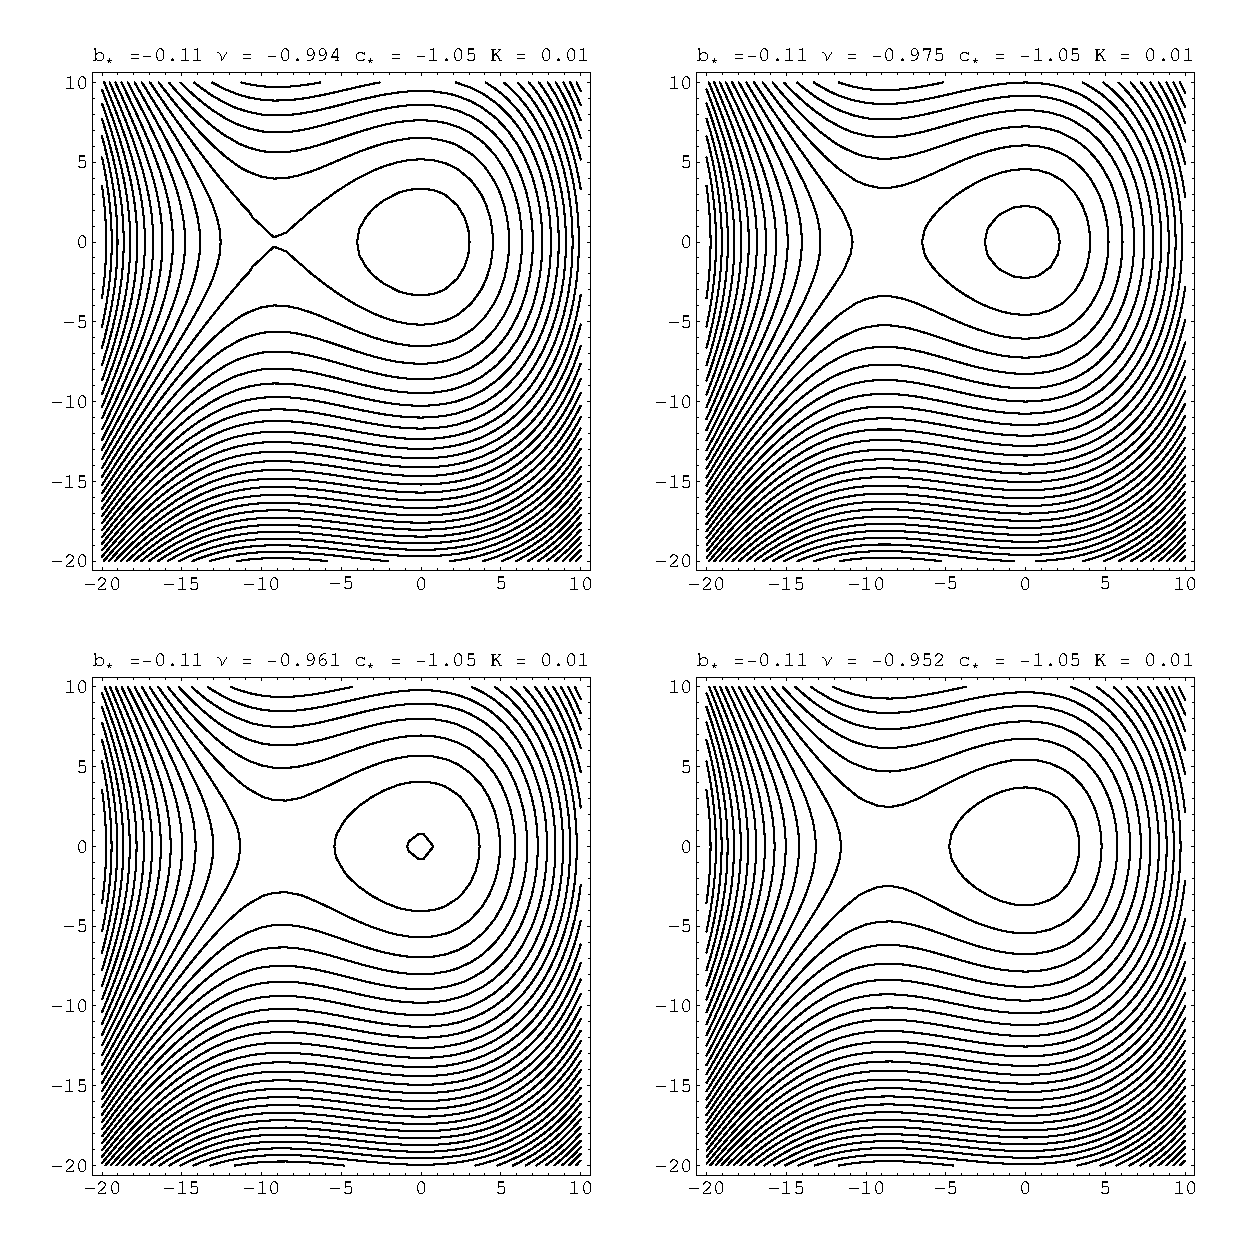
\includegraphics[width=1.0\textwidth]{figures/figure2-1c}
\label{fig:homoclinic2} \caption{Level curves of \eqref{eq:H} corresponding to
various values of H.} \end{center} \end{figure}
  %% everytime u use include it starts at the top of the new page, so it's good for chapters
\chapter{CHAPTER THREE: A Microstructure PDE } \label{chapter_3}

\section{Introduction}

One dimensional wave propagation in microstructured solids is currently a topic of great interest.
This phenomenon has recently been modeled \cite{STE} by an equation

\begin{equation}\label{eq:MS}
v_{tt} - b v_{xx} - \frac{\mu}{2} \left( v^2 \right)_{xx} - \delta \left( \beta v_{tt} - \gamma v_{xx}\right)_{xx} = 0 
\end{equation}
with complicated dispersive and nonlinear terms. Here $b, \mu, \beta, \delta$
and $\gamma$ are dimensionless parameters, $v$ denotes the macrodeformation,
and $x$ and $t$ denote space and time coordinates respectively.

Equation \eqref{eq:MS} is derived, using the so-called Mindlin Model, in
\cite{STE}, \cite{JE1}, \cite{JE2}.  It is non-integrable. However, analytic
conditions for the existence of solitary waves of \eqref{eq:MS} have been
derived in \cite{JE2} and \cite{STE}. These references also numerically
construct asymmetric solitary wave solutions of the form $ v\left(x - c t
\right)$ of \eqref{eq:MS}.  More recently (\cite{EP},\cite{EBS}) pulse trains
in \eqref{eq:MS} have been numerically constructed.

\section{Solitary waves; local bifurcations}


Solitary waves of \eqref{eq:MS} of the form 
$v(x,t) = \phi\left(x - c t\right) = \phi\left(z\right)$
 satisfy the fourth-order traveling wave ODE
\begin{equation} \label{eq:ode2} \phi_{zzzz} - q \phi_{zz} + p \phi = \mathcal{N}[\phi]
\end{equation}

where 
% the notation $\mathcal{N[\phi]}$ means that the operator $\mathcal{N}$ operates on $\phi$ and all of it's derivatives, and 
\begin{equation}
\mathcal{N}\left[\phi\right] = -\Delta_1 \phi_z^2 - b \Delta_1 \phi \phi_{zz}
\end{equation}

%where 
\begin{subequations}
\begin{eqnarray}
z &\equiv& x - c t\\
p &\equiv& 0\label{eq:pdef} \\
q &\equiv & \frac{c^2 - b}{\delta\left(\beta c^2 - \gamma\right)} 
\label{eq:qdef2} \\
\Delta_1 &\equiv& \frac{\mu}{ \delta\left( \beta c^2 - \gamma\right) }\label{eq:deltadef} 
\end{eqnarray}
\end{subequations}
Equation \eqref{eq:ode2} is invariant under the transformation $ z \mapsto -z $ and is thus a reversible system. In this section we shall
use the theory of reversible systems to characterize the homoclinic orbits to the fixed point of \eqref{eq:ode2}, which correspond to pulses
or solitary waves of \eqref{eq:MS} in various regions of the $(p,q)$ plane.

The linearized system corresponding to \eqref{eq:ode2}
\begin{equation}
 \label{eq:linode2} \phi_{zzzz} - q \phi_{zz} + p \phi = 0
\end{equation}
has a fixed point \begin{equation}\label{eq:fp2} \phi = \phi_z = \phi_{zz} = \phi_{zzz} = 0 \end{equation}

Solutions $\phi = k e^{\lambda x}$ satisfy the characteristic equation
$\lambda^4 - q \lambda^2 + p = 0 $ from which one may deduce that the structure
of the eigenvalues is distinct in two regions of $\left(p,q\right)$-space.
Since $p=0$ we have only two possible regions of eigenvalues.  We denote $C_0$
as the positive $q$ axis and $C_1$ the negative $q$-axis. First we shall 
consider the bounding curves $C_0$ and $C_1$ and their neighborhoods, then we shall discuss the possible
occurrence and multiplicity of homoclinic orbits to \eqref{eq:fp2}, corresponding
to pulse solitary waves of \eqref{eq:MS}, in each region:

\begin{description}
\item[Near $C_0$] 
The eigenvalues have the structure $\lambda_{1-4} = 0,0,\pm \lambda$, ($\lambda \in \mathbb{R}$) and the fixed point
\eqref{eq:fp} is a saddle-focus.
\item[Near $C_1$] 
Here the eigenvalues have the structure $\lambda_{1-4} = 0,0,\pm i \omega $, ($\omega \in \mathbb{R}$) . We will show by analysis of a
four-dimensional normal form in Section 4 that there exists a $\mathrm{sech}^2$ homoclinic orbit near $C_1$.
\end{description}

Having outlined the possible families of orbits homoclinic to the fixed point \eqref{eq:fp} of \eqref{eq:linode2},
corresponding to pulse solitary waves of \eqref{eq:MS}, we now derive normal forms near the transition curves $C_0$ and $C_1$
to confirm the existence of regular or delocalized solitary waves in the corresponding regions of $\left(p,q\right)$ parameter space.

\section{Normal form near $C_0$: solitary wave solutions}

Using \eqref{eq:linode2}, the curve $C_0$, corresponding to $\lambda = 0,0,\pm \tilde{ \lambda } $, is given by
\begin{equation}
C_0: { p=0, q > 0 }
\end{equation}

Using \eqref{eq:qdef2} implies
\begin{equation}
 \frac{c^2 - b}{\delta\left(\beta c^2 - \gamma\right)} > 0
\end{equation}

Denoting $\phi$ by $y_1$, equation \eqref{eq:ode2} may be written as the system
\begin{subequations}\label{eq:system2}
\begin{eqnarray}
\frac{d y_1 }{d z} &=& y_2 \\
\frac{d y_2 }{d z} &=& y_3 \\
\frac{d y_3 }{d z} &=& y_4 \\
\frac{d y_4 }{d z} &=& q y_3 - p y_1 - \left(\Delta_1 y_2^2 + b \Delta_1 y_1 y_3 \right)
\end{eqnarray}
\end{subequations}

We wish to rewrite this as a first order reversible system in order to invoke the relevant theory \cite{IA}. 
To that end, defining  $Y=\left<y_1,y_2,y_3,y_4\right>^T$, equation \eqref{eq:system2} may be written 

\begin{equation}\label{eq:bilinear2}
\frac{ dY }{ dz } = L_{pq} Y - F_2(Y,Y)
\end{equation}

where 
\begin{equation}
L_{pq} = \left( 
\begin{array}{cccc}
0&1&0&0\\
q/3&0&1&0\\
0&q/3&0&1\\
q^2 - p &0&q/3&0 \end{array} \right) \end{equation}

Since $p=0$ for \eqref{eq:MS}, we have 
\begin{equation} \label{eq:bilinear2}
 \frac{ dY }{ dz } = L_{0q} Y - F_2(Y,Y) 
\end{equation}
where 
\begin{equation}\label{eq:nonlinear2}
F_2(Y,Y) = \left<0,0,0,\Delta_1 y_2^2 + b \Delta_1 y_1 y_3 \right>^T
\end{equation}

Next we calculate the normal form of \eqref{eq:bilinear2} near $C_0$. The procedure is
closely modeled on \cite{IA} and many intermediate steps may be found there. 

\subsection{ Near $C_0$ }
Near $C_0$ the dynamics reduce to a two-dimensional Center Manifold
\begin{equation}\label{eq:c0cm2}
 Y = A \zeta_0 + B \zeta_1 + \Psi(\epsilon,A,B)
\end{equation}
and the corresponding normal form is
\begin{subequations}\label{eq:c0nf2}
\begin{eqnarray}
\frac{dA}{dz} &=& B \label{eq:c0nf2a} \\
\frac{dB}{dz} &=& b \epsilon A + \tilde{c} A^2 \label{eq:c0nf2b}
\end{eqnarray}
\end{subequations}
Here,
\begin{equation}
\epsilon = \left( \frac{q^2}{9} - p\right) - \left(\frac{q}{3}\right)^2 = - p 
\end{equation}
measures the perturbation around $C_0$, and

\begin{subequations}\label{eq:lineareigs2}
\begin{eqnarray}
\zeta_0 &=& \left<1,0,-q/3,0\right>^T\\
\zeta_1 &=& \left<0,1,0,-2 q/3\right>^T 
\end{eqnarray}
\end{subequations}

The linear eigenvalue of \eqref{eq:c0nf2} satisfies 
\begin{equation}\label{eq:lineig2}
\lambda^2 = b \epsilon 
\end{equation}
The characteristic equation of the linear part of 
\eqref{eq:bilinear2} is 
\begin{equation}\label{eq:charlinear2}
\lambda^4 - q \lambda^2 - \epsilon =  0 
\end{equation}
Hence, the eigenvalues near zero (the Center Manifold) satisfy $\lambda^4 \ll \lambda^2$ and hence 
\begin{equation}\label{eq:lindominant2}
\lambda^2 \sim -\frac{\epsilon}{q}
\end{equation}
Matching \eqref{eq:lineig2} and \eqref{eq:lindominant2} 
\begin{equation}
b = - \frac{1}{q}
\end{equation}
and only the nonlinear coefficient $\tilde{c}$ remains to be determined in the normal form \eqref{eq:c0nf2}.

In order to determine $\tilde{c}$ (the coefficient of $A^2$ in \eqref{eq:c0nf2})
we calculate $\frac{dY}{dz}$ in two ways and match the $\mathcal{O}(A^2)$
terms.  To this end, using the standard 'suspension' trick of treating the
perturbation parameter $\epsilon$ as a variable, we expand the function $\Psi$
in \eqref{eq:c0cm2} as 

\begin{equation}\label{eq:psiexp2}
\Psi(\epsilon,A,B) = \epsilon A \Psi_{10}^1 + \epsilon B \Psi_{01}^1 + A^2 \Psi_{20}^0 + A B \Psi_{11}^0 + B^2 \Psi_{02}^0 + \cdots
\end{equation}
where the subscripts denote powers of $A$ and $B$, respectively, and the superscript denotes the power of $\epsilon$. 

In the first way of computing $dY/dz$, we take
the $z$ derivative of \eqref{eq:c0cm2} (using \eqref{eq:c0nf2} and \eqref{eq:psiexp2}). 
The coefficient of $A^2$ in the resulting expression is $\tilde{c} \zeta_1 $. In the second way of computing $dY/dz$, we use \eqref{eq:c0cm2} and \eqref{eq:psiexp2} in \eqref{eq:bilinear2}. The coefficient of $A^2$ in the resulting expression is 
$ L_{0,q} \Psi_{20}^0 - F_2\left(\zeta_0,\zeta_0\right)$.  Hence
\begin{equation}\label{eq:A2coef2}
 \tilde{c} \zeta_1 = L_{0q} \Psi_{20}^0 - F_2(\zeta_0,\zeta_0) \end{equation}

Using \eqref{eq:lineareigs2} and \eqref{eq:nonlinear2} and denoting $\Psi_{20}^0 = \left<x_1,x_2,x_3,x_4\right>$ in \eqref{eq:A2coef2} yields the equations

\begin{subequations}
\begin{eqnarray}
0 &=& x_2 \\
\tilde{c} &=& \frac{q}{3} x_1 + x_3 \label{eq:A2coef2b}\\
0 &=& \frac{q}{3} x_2 + x_4 \implies x_4 = 0
\textrm{ using \eqref{eq:A2coef2b} }
\end{eqnarray}
\end{subequations}
and
\begin{equation}
-\frac{2q}{3} \tilde{c} = \frac{q}{3}\left(\frac{q}{3} x_1 + x_3 \right) + \frac{2q}{3} = \frac{q}{3} \tilde{c} + \frac{b \Delta_1 }{3} 
\textrm{ using \eqref{eq:A2coef2b} }
\end{equation}
Hence we obtain 
\begin{equation}
\tilde{c} = - \frac{b \Delta_1}{3} 
\end{equation}
 
Therefore, the normal form for \eqref{eq:MS} near $C_0$ is
\begin{subequations}
\begin{eqnarray}
\frac{dA}{dz} &=& B \\
\frac{dB}{dz} &=& -\frac{\epsilon}{q} A - \frac{ b \Delta_1}{3}  A^2
\end{eqnarray}
\end{subequations}

The normal form \eqref{eq:c0nf2} admits a homoclinic solution (near $C_0$) of the form 
\begin{equation} \label{eq:ms_soliton1}
A\left(z\right) = \ell \space \mathrm{sech}^2\left(k z\right)
\end{equation}

with 
\begin{subequations} 
\begin{eqnarray}
k &=& \sqrt{\frac{-\epsilon}{4q}} \label{eq:keq2} \\
\ell &=& \frac{ 6 k^2 }{ b \Delta_1 } 
\end{eqnarray}
\end{subequations}


Hence, since $\epsilon = - p $, and the curve $C_0$ corresponds to $p=0,q>0$, solitary waves of the 
form \eqref{eq:ms_soliton1} exist in the vicinity of $C_0$ for 
\begin{equation}
p > 0, q > 0 
\end{equation}
which implies that $  \frac{c^2 - b}{\delta\left(\beta c^2 - \gamma\right)} > 0 $
(such that $k$ in \eqref{eq:keq2} is real.)  As mentioned in section 2, one may show the persistence
of this homoclinic solution in the original traveling wave ODE \eqref{eq:linode2}. Thus, we have 
demonstrated the existence of solitary waves of \eqref{eq:MS} for $p=0^+, q>0$. 

\section{Normal form near $C_1$: possible solitary wave solutions}
Using \eqref{eq:linode2}, the curve $C_1$, corresponding to $\lambda = 0, 0\pm i \omega$, is given by
\begin{equation}\label{eq:ms_c1}
C_1 : { p = 0, q < 0 }
\end{equation}
Which implies
\begin{equation}
\frac{c^2 - b}{ \delta\left(\beta c^2 - \gamma \right)} < 0
\end{equation}

In order to investigate the possibility of a $ \mathrm{sech}^2 $  homoclinic orbit in
the neighborhood of $C_1$ and delocalized solitary waves, we next compute the
normal form near $C_1$ following the procedure in \cite{IA}.

Near $C_1$ the dynamics reduce to a four-dimensional Center Manifold \cite{IA}.
Since all the eigenvalues are non-hyperbolic, the Center Manifold has the form
(a nonlinear coordinate change \cite{IA})
\begin{equation} \label{eq:c1cm2}
Y = A \zeta_0 + B \zeta_0 + C \zeta_+ + \bar{C} \zeta_- + \Psi(\epsilon,A,B,C,\bar{C})
\end{equation}

with  a corresponding four-dimensional normal form
\begin{subequations}\label{eq:c1nf}
\begin{eqnarray}
\frac{dA}{dz} &=& B \label{eq:aq2} \\
\frac{dB}{dz} &=& \bar{\nu} A + b_* A^2 + c_* \left|C\right|^2  \label{eq:bq2} \\
\frac{dC}{dz} &=& i d_0 C + i \bar{\nu} d_1 C + i d_2 A C \label{eq:cq2}
\end{eqnarray}
\end{subequations}
Here $C$ is complex, $\bar{C}$ is the complex conjugate of $C$, $\epsilon,
\zeta_0, \zeta_1$ are given previously and the two new complex eigenvectors
co-spanning the Center Manifold are
\begin{equation}
\zeta_\pm	 = \left< 1, \lambda_\pm, 2 q / 3, \frac{\lambda_\pm}{3} q\right>^T 
\end{equation}

Using \eqref{eq:bq2} and \eqref{eq:c0nf2b}
\begin{equation}
\bar{\nu} = b \epsilon = -\frac{\epsilon}{q} 
\end{equation}

Also from the characteristic equation \eqref{eq:charlinear2}, the two non-zero 
(imaginary) roots are 
\begin{equation}
\lambda^2 = \frac{ q + \sqrt{q^2 + 4 \epsilon } }{2} \approx q \textrm{ for } \epsilon \textrm{ small }
\end{equation}

Hence
\begin{equation}
\lambda = \pm i \sqrt{-q}, q < 0
\end{equation}

Matching this to the linear part of \eqref{eq:cq2} ( which corresponds to the
imaginary eigenvalues), $\lambda = i d_0 = i \sqrt{-q}$ or 
\begin{equation}
d_0 = \sqrt{-q}
\end{equation}


With a dominant balance argument after the change of variable $\epsilon =
\sqrt{-3 \alpha}$ on the characteristic equation \eqref{eq:charlinear2} as $\lambda \rightarrow 0 $ we
find $d_1 = \frac{ \sqrt{-3 \alpha} }{18 \alpha^2 } $. Using $\alpha=q/3$
implies 
\begin{equation}
d_1 = \frac{\sqrt{-q}}{2 q^2}
\end{equation}

The remaining undetermined coefficients  in the normal form are the 
coefficients $b_*,c_*$ and $d_2$ 
which correspond to the $A^2, |C|^2$ and $AC$ terms respectively. In 
order to determine them, we follow the same procedure as 
in Section 3 and compute $dY/dz$ is two distinct ways. We expand the
function $\Psi$ as
\begin{equation}\label{eq:psiexp2}
\Psi(\epsilon,A,B,C,\bar{C}) = \epsilon A \Psi_{1000}^1 + \epsilon B \Psi_{0100}^1 + A^2 \Psi_{2000}^0 + A B \Psi_{1100}^0 + A C \Psi_{1010}^0 + \epsilon C \Psi_{0010}^1 + \cdots 
\end{equation}

with subscripts denoting powers of $A$, $B$, $C$ and $\bar{C}$, respectively,
and the superscript is the power of $\epsilon$. In the first way, $dY/dz$ is
computed by taking the $z$ derivative of \eqref{eq:c1cm2} (using \eqref{eq:c1nf2}
and \eqref{eq:psiexp2}) and read off the coefficients of $A^2, \|C\|^2, C
\epsilon$ and $AC$ terms.  In the second way, $dY/dz$ is computed using
\eqref{eq:c1cm2} and \eqref{eq:psiexp2} in \eqref{eq:bilinear2} (with $p=0$ on
$C_1$ as given in \eqref{eq:ms_c1}) and the coefficients of  $A$, $B$, $C$ and
$\bar{C}$ are once again read off.  Equating the coefficients of the
corresponding terms in the two separate expressions for $dY/dz$ yields the
following equations:

\begin{subequations}
\begin{eqnarray}
\mathcal{O}(A^2): &		b_* \zeta_1 &= L_{0q} \Psi_{2000}^0 - F_2(\zeta_0,\zeta_0) \\
\mathcal{O}(\left|C\right|^2):&	c_* \zeta_1 &= L_{0q} \Psi_{0011}^0 -2 F_2(\zeta_+,\zeta_-) \label{eq:cstar2} \\
\mathcal{O}(\epsilon C): &-\frac{i}{q} \left(d_1 \zeta_+ +  d_0 \Psi_{0010}^1\right) &= L_{0q} \Psi_{0010}^1 - F_2(\Psi_{0010}^1,\Psi_{0010}^1) \\
\mathcal{O}(A C): 	&i d_2 \zeta_+ + i d_0 \Psi_{1010}^0 &= L_{0q} \Psi_{1010}^0 - 2 F_2(\zeta_0,\zeta_+) \label{eq:AC2}
\end{eqnarray}
\end{subequations}
where we have used the fact that $F_2$ is a symmetric bilinear form. Equation \eqref{eq:cstar} is decoupled and yields 
$ c_* = 2 \Delta_1 \left( \frac{2 b}{3}  - 1\right)$. The only coefficient left to determine is $d_2$ which we shall compute now. 

Using $\Psi_{1010}^0 = \left<x_1,x_2,x_3,x_4\right>^T$ in \eqref{eq:AC2} implies 

\begin{subequations}
\begin{eqnarray}
i d_2 + i d_0 x_1 &=& x_2 \label{eq:one2} \\
- d_0 d_2 + i d_0 x_2 &=& \frac{q}{3} x_1 + x_3 \label{eq:two2} \\
\frac{2 i q}{3} d_2 + i d_0 x_3 &=& \frac{q}{3} x_2 + x_4  \label{eq:three2} \\
- \frac{q}{3} d_0 d_2 + i d_0 x_4 &=& \frac{q}{3}\left(\frac{q}{3} x_1 + x_3 \right) - \frac{ 2 b q \Delta_1} {3} \label{eq:four2}
\end{eqnarray}
\end{subequations}

Using \eqref{eq:one2} in \eqref{eq:two2} , \eqref{eq:two2} in \eqref{eq:four2} and
using these in \eqref{eq:three2} yields $ d_2 = \frac{ b \Delta_1 }{ 3 \sqrt{-q} }$.

Therefore the normal form for \eqref{eq:MS} near $C_1$ is 

\begin{subequations}\label{eq:NORMAL2}
\begin{eqnarray} 
\frac{dA}{dz} &=& B  \label{eq:normalA2} \\
\frac{dB}{dz} &=& -\frac{\epsilon}{q} A - \frac{b \Delta_1 }{3} A^2 + 2 \Delta_1 \left(\frac{2 b }{3} - 1\right) \left|C\right|^2  \label{eq:normalB2} \\
\frac{dC}{dz} &=& i \sqrt{-q} C - i \frac{\sqrt{-q} }{q^3} C\epsilon + i \frac{b \Delta_1}{3 \sqrt{-q}} A C \label{eq:normalC2}
\end{eqnarray}
\end{subequations}

The dynamics inherent in \eqref{eq:NORMAL2} may be elucidated following the
discussions of \cite{IA}, \cite{IK}, \cite{Lombardi1} and \cite{Lombardi2}.
The two first integrals of \eqref{eq:c1nf2}  are
\begin{equation}
K = \left| C \right|^2
\end{equation}
and
\begin{equation}\label{eq:H2}
H = B^2 - \frac{2}{3} b_* A^3 - \bar{\nu} A^2 - 2 c_* K A
\end{equation}
Also, $c_*$ should be real  for the following energy arguments to apply.
As a typical case, consider  the level curve $H=0$ of the energy-like first
integral function $H$. In the $(A,B)$ phase plane, this will compromise a
homoclinic orbit. The intersection of $H=0$ with the $A$ axis occurs for $
\frac{2}{3} b_* A^2 - \bar{\nu}A - 2 c_* K = 0$ or
\begin{equation}
A_{\mp} = \frac{3}{4 b_*} \left[ \bar{\nu} \pm \sqrt{ \bar{\nu}^2 + \frac{16 b_* c_* K}{3} } \right]
\end{equation}
Note that $A_+ > 0, A_- < 0 $ for $b_* c_* > 0 $ and $b_* < 0$ as relevant for
us. A general homoclinic orbit, homoclinic to $A_+$, is sketched in Figure 1
where the flow direction is deduced from \eqref{eq:normalA2}.  For
$K=\left|C\right|^2 = 0 $, the orbit is homoclinic to $A_+=0$. For small
non-zero $\left|K\right|$, $ A_+ \sim - 2 c_* K / \bar{\nu}$, meaning that
oscillations at infinity are then very small in this case. For $K=0$ this
corresponds to an \emph{orbit homoclinic to} 0 for the normal form. This is indeed
valid for the normal form taken at any order. However this solution does not
exist mathematically for the full original system, even though one may compute
its expansion in powers of the bifurcation parameter up to any order (see
\cite{Lombardi1} and \cite{Lombardi2}). This is an example of the famous
challenging problem of asymptotics beyond any orders. Other solutions found on
the normal form mainly persist under the perturbation from higher order terms
provided by the original system \cite{IK}. These solutions are delocalized
waves and their existence in Region 2 is guaranteed by the general theory for
reversible systems in \cite{Lombardi1} and \cite{Lombardi2}. Also, as mentioned
in Section 2, genuine solitary waves are found on isolated curves in Region 2
of Figure 1 on which the oscillation amplitudes vanish. Since these are
embedded in the sea of delocalized solitary waves and in the continuous
spectrum, they are referred to as embedded solitons \cite{CMYK}. These will
further be investigated in Region 2 subsequently using a mix of exponential
asymptotics and numerical shooting.

\begin{figure}[hh]
\begin{center}
\label{fig:homoclinic3}
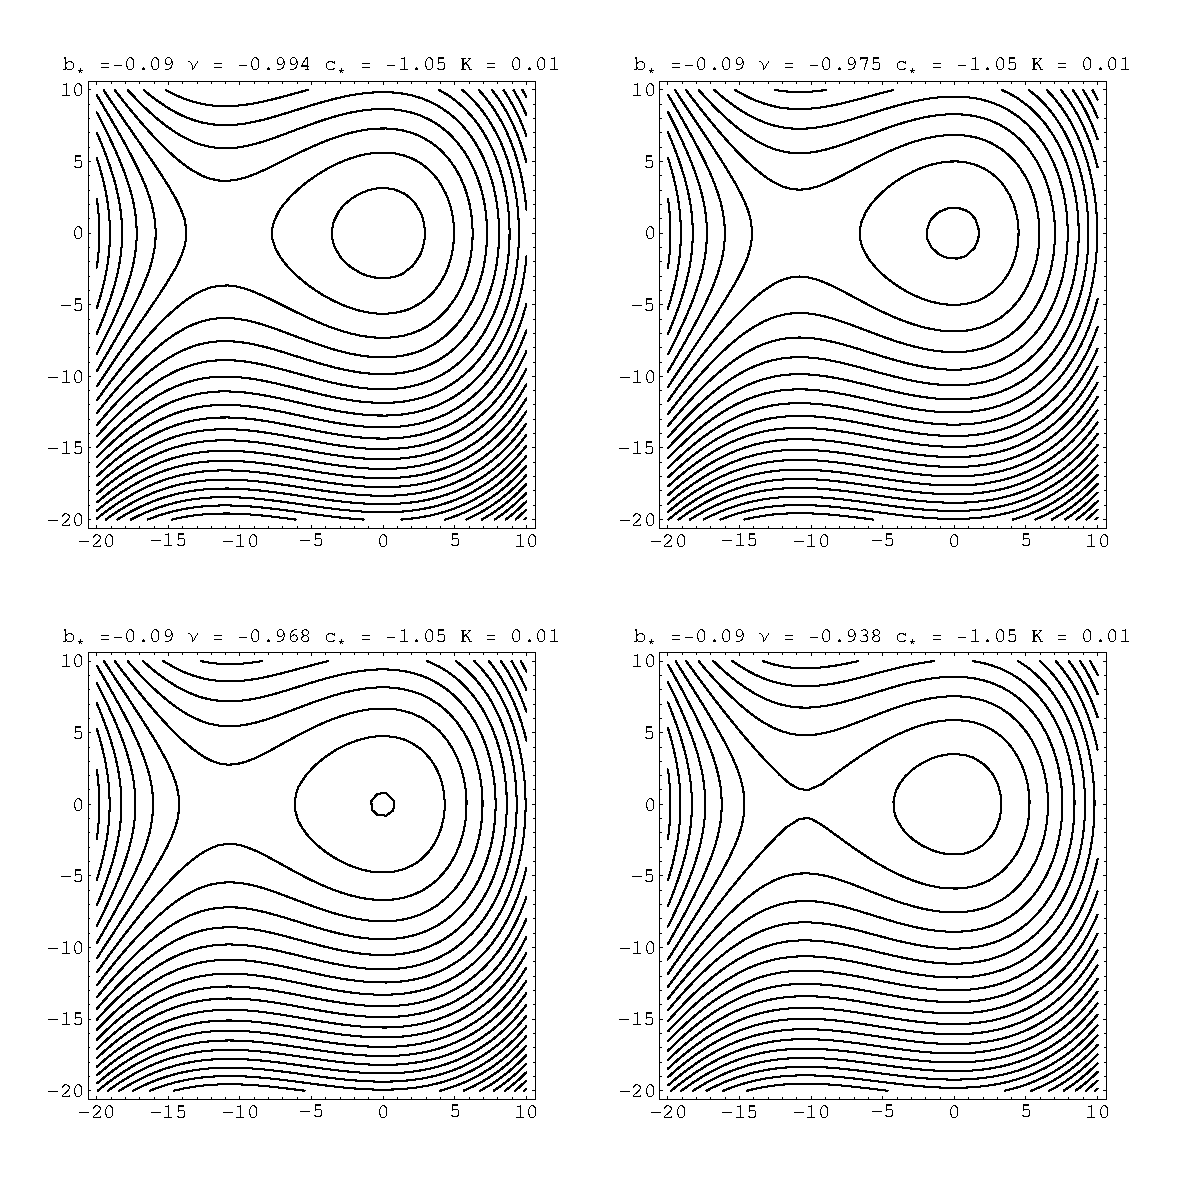
\includegraphics[width=1.0\textwidth]{figures/figure3-1a}  
\caption{Level curves of \eqref{eq:H2} corresponding to various values of H.}
\end{center}
\end{figure}



\chapter{CHAPTER FOUR: FINDINGS} \label{chapter_4}


Chapter Four, also called �Results� or �Data Analysis,� usually provides detailed findings of the research. This chapter is where tables and figures most often appear, so make sure formatting is consistent.

\section{Sample Table}

The following sample table is an example of acceptable table formatting. Descriptive titles appear above tables and may appear either on one line or stacked and single-spaced. The table itself may also be single-spaced as necessary.
If possible, try to keep tables and/or figures all on one page. If necessary, start the table or figure on a new page, even if this means leaving blank space on the preceding page. If you must split a table over multiple pages, repeat the table headings and continue. It is not necessary to repeat the table title.

\begin{table}[!ht] \singlespacing
\caption{Classroom Checklist for Physical Organization (a sample table)} \label{tbl:my_first_table}
\begin{center}
\begin{tabular}{lcccccc}
 & \multicolumn{6}{c}{Classrooms} \\ \hline
Physical Components & A & B & C & D & E & F \\
Desk Groupings for Student Interaction & 5 & 3 & 3 & 5 & 3 & 2 \\
Learning and Resource Centers & 3 & 2 & 2 & 3 & 1 & 1 \\
Flexibility of Furniture Use & 3 & 4 & 3 & 3 & 2 & 1 \\
Specific M/G Displays & 1 & 1 & 3 & 2 & 2 & 2 \\
Total out of 30 points & 12 & 10 & 11 & 13 & 8 & 6 \\ \hline
\end{tabular}
\end{center}
\vspace{-4ex}
\begin{minipage}{\textwidth}
\singlespacing \footnotesize \flushleft
Degree of Application: 5=High; 4=Medium-High; 3=Medium; 2=Medium-Low; 1=Low
M/G=Multicultural/Global

\noindent A, B, C, D, E, and F are the classrooms of Alice, Betty, Carol, Donna, Elaine, and Fran respectively.
\end{minipage}
\end{table}

\section{Sample Figure}

The following is a sample figure with acceptable figure formatting. For figures, be sure you format both the figure and the figure title consistently. This includes placement (centered or left-justified), spacing before and after, line spacing, point size and font.

\begin{figure}[!ht] \singlespacing
\begin{center}
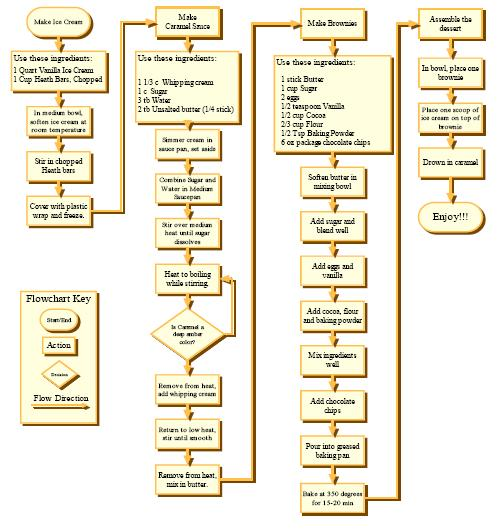
\includegraphics[width=.8\textwidth]{figures/figure_1}  %% good idea to keep your figures in a separate folder
\end{center}
\caption{Heath Bar Caramel Brownie Sundae} \label{tbl:my_first_figure}
\end{figure}

%% Best way to generate pictures, especially graphs, is to save them (say from MATLB) as .eps (Encapsulated PostScript) and than
%% convert to PDF using (attached) eps2pdf utility. Note that pdfTeX will not accept .eps files.
\chapter{CHAPTER FIVE: CONCLUSION} \label{chapter_5}

Chapter Five, also called ``Summary'', ``Conclusion'' or ``Recommendations'', usually presents a conclusion to the research, offers recommendations to the problem investigated, or discusses implications for future studies.

\section{Bookmarks}

A few words about bookmarks. Frontmatter entries, like the Abstract, Acknowledgments and the Table of Contents should appear in the bookmarks �� but not in the Table of Contents. The TOC contains only pages that appear after the Table of Contents in the document, usually beginning with the List of Figures. So, bookmark and Table of Contents entries do vary.
However, bookmarks should include all major and chapter headings and at least first-level subheadings EXACTLY as they appear in the document (and the TOC). And readers should be able to link to pages within the ETD from all of the bookmarks, the TOC entries, as well as the Lists of Figures and Tables.

\appendix  %% just makes "Chapter" to be called "Appendix"

\chapter{APPENDIX: TITLE OF APPENDIX} \label{appendix_A}

%% if you have only one appendix the header should read:
%\chapter{APPENDIX: TITLE OF APPENDIX} \label{appendix_A}
%\addcontentsline{toc}{chapter}{APPENDIX}

\newpage

\begin{itemize}
\item Begin appendix text on the page following the buffer page
\item Continue Arabic pagination; do not restart page numbering with an appendix
\item Use the same style and format for buffer page headings as you do for other body chapter headings.
\item Letter, don�t number, appendixes (e.g., APPENDIX A, APPENDIX B)
\item If you have only one appendix, do not letter it at all
\item Appendixes should follow the margin and other formatting requirements from the rest of the document
\end{itemize}

\section{About References}

References appear in the style of your particular reference system. While a hanging indent is preferred, some style guides use alternate formatting.
References should be either double-spaced throughout, with no space between entries, or single-spaced within entries with a double space between.
Below find a sample reference with a hanging indent, formatting along APA style. Here is how to cite:~\cite{Allison_2000}.  
\chapter{APPENDIX B: TITLE OF APPENDIX} \label{appendix_B}

\newpage

\begin{itemize}
\item Begin appendix text on the page following the buffer page
\item Continue Arabic pagination; do not restart page numbering with an appendix
\item Use the same style and format for buffer page headings as you do for other body chapter headings.
\item Letter, don�t number, appendixes (e.g., APPENDIX A, APPENDIX B)
\item If you have only one appendix, do not letter it at all
\item Appendixes should follow the margin and other formatting requirements from the rest of the document
\end{itemize}

\section{About References}

References appear in the style of your particular reference system. While a hanging indent is preferred, some style guides use alternate formatting.
References should be either double-spaced throughout, with no space between entries, or single-spaced within entries with a double space between.
Below find a sample reference with a hanging indent, formatting along APA style. Here is how to cite:~\cite{Allison_2000}.  %% you may have more than one appendix, use letters to distingush among them

\bibliographystyle{plain} %% you can choose different bibliography style and the rest ia all automatic
\bibliography{references} %% this is your database with literature

\end{document}